\documentclass[../main.tex]{subfiles}

\usepackage{caption}
\captionsetup[table]{name=New asdasdqw}


\begin{document} 
\chapter{Adaptive methods and Stiff Systems}\label{chap:chap23}

\begin{center}
    \Large{\textbf{CHAPTER OBJECTIVES}}
\end{center}
The primary objective of this chapter is to introduce you to more advanced methods
for solving initial-value problems for ordinary differential equations. Specific
objectives and topics covered are:
\begin{itemize}
    \item Understanding how the Runge-Kutta Fehlberg methods use RK methods of
    different orders to provide error estimates that are used to adjust the step size.
    \item Familiarizing yourself with the built-in MATLAB functions for solving ODEs
    \item Learning how to adjust the options for MATLAB's ODE solvers
    \item Learning how to pass parameters to MATLAB's ODE solvers.
    \item Understanding the difference between one-step and multistep methods for solving
    ODEs.
    \item Understanding what is meant by stiffness and its implications for solving ODEs.
    \end{itemize}
\vspace{2cm}
\section{Adaptive Runge-Kutta methods}
To this point, we have presented methods for solving ODEs that employ a constant step size.
For a significant number of problems, this can represent a serious limitation. For example,
suppose that we are integrating an ODE with a solution of the type depicted in Fig. 23.1. For
most of the range, the solution changes gradually. Such behavior suggests that a fairly large
step size could be employed to obtain adequate results. However, for a localized region from
$t$ = 1.75 to 2.25, the solution undergoes an abrupt change. The practical consequence of
dealing with such functions is that a very small step size would be required to accurately
capture the impulsive behavior. If a constant step-size algorithm were employed, the smaller
step size required for the region of abrupt change would have to be applied to the entire computation. As a consequence, a much smaller step size than necessary and, therefore, many
more calculations-would be wasted on the regions of gradual change.

Algorithms that automatically adjust the step size can avoid such overkill and hence be
of great advantage. Because they ``adapt'' to the solution's trajectory, they are said to have $adaptive$ $step-size control$. Implementation of such approaches requires that an estimate of
the local truncation error be obtained at each step. This error estimate can then serve as a
basis for either shortening or lengthening the step size.

Before proceeding, we should mention that aside from solving ODEs, the methods
described in this chapter can also be used to evaluate definite integrals. The evaluation of
the definite integral
\begin{equation}
    I=\int_{a}^{b} f(x) dx   \nonumber 
\end{equation}


is equivalent to solving the differential equation
\begin{equation}
    \frac{dy}{dx} = f(x)    \nonumber
\end{equation}

for y (b) given the initial condition y (a) = 0. Thus, the following techniques can be em-
ployed to efficiently evaluate definite integrals involving functions that are generally
smooth but exhibit regions of abrupt change.

\begin{figure}[H]
    \centering
    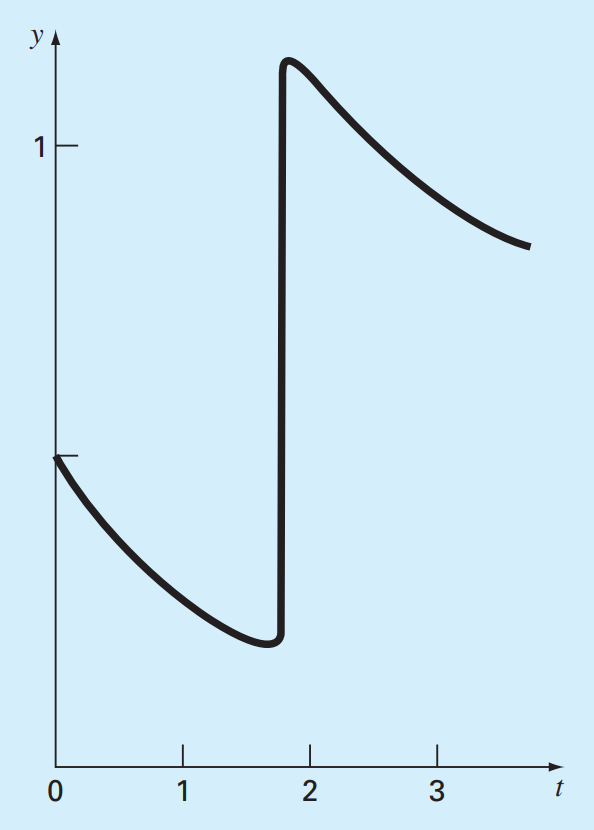
\includegraphics[scale=0.4]{fig_23_1}
   \caption{\textsf{An example of a solution of an ODE that exhibits an abrupt change. Automatic step-size adjustment has great advantages for such cases.}}\label{fig:fig_23_1}
\end{figure}
There are two primary approaches to incorporate adaptive step-size control into one-
step methods. Step halving involves taking each step twice, once as a full step and then as
two half steps. The difference in the two results represents an estimate of the local trunca-
tion error. The step size can then be adjusted based on this error estimate.

In the second approach, called embedded RK methods, the local truncation error is estimated as the difference between two predictions using different-order RK methods. These
are currently the methods of choice because they are more efficient than step halving.

The embedded methods were first developed by Fehlberg. Hence, they are sometimes
referred to as $RK-Fehlberg methods$. At face value, the idea of using two predictions of different order might seem too computationally expensive. For example, a fourth-and fift-horder prediction amounts to a total of 10 function evaluations per step [recall Eqs. (22.44)
and (22.45)]. Fehlberg cleverly circumvented this problem by deriving a fifth-order RK
method that employs most of the same function evaluations required for an accompanying
fourth-order RK method. Thus, the approach yielded the error estimate on the basis of only
six function evaluations!

\subsection{MATLAB Function for Nonstiff System}

Since Fehlberg originally developed his approach, other even better approaches have been
developed. Several of these are available as built-in functions in MATLAB.\

\textbf{ode23.} The \texttt{ode23} function uses the BS23 algorithm (Bogacki and Shampine, 1989;
Shampine, 1994), which simultaneously uses second- and third-order RK formulas to solve
the ODE and make error estimates for step-size adjustment. The formulas to advance the
solution are
\begin{equation}
    \tag{23.1}
    y_{i+1}=y_{i}+\frac{1}{9}\left(2 k_{1}+3 k_{2}+4 k_{3}\right) h
\end{equation}
where
\begin{equation}
    \tag{23.1$a$}
    k_{1}=f\left(t_{i}, y_{i}\right)
\end{equation}
\begin{equation}
    \tag{23.1$b$}
    k_{2}=f\left(t_{i}+\frac{1}{2} h, y_{i}+\frac{1}{2} k_{1} h\right)\\
\end{equation}
\begin{equation}
    \tag{23.1$c$}
    k_{3}=f\left(t_{i}+\frac{3}{4} h, y_{i}+\frac{3}{4} k_{2} h\right)\\
\end{equation}
The error is estimated as\
\begin{equation}
    \tag{23.2}
    E_{i+1}=\frac{1}{72}\left(-5 k_{1}+6 k_{2}+8 k_{3}-9 k_{4}\right) h
\end{equation}
where
\begin{equation}
    \tag{23.2$a$}
    k_{4}=f\left(t_{i+1}, y_{i+1}\right)
\end{equation}
Note that although there appear to be four function evaluations, there are really only three
because after the first step, the $k1$ for the present step will be the $k4$ from the previous step.
Thus, the approach yields a prediction and error estimate based on three evaluations rather
than the five that would ordinarily result from using second- (two evaluations) and thirdorder (three evaluations) RK formulas in tandem

After each step, the error is checked to determine whether it is within a desired tolerance. If it is, the value of $y\textsubscript{i+1}$ is accepted, and $k4$ becomes $k1$ for the next step. If the error
is too large, the step is repeated with reduced step sizes until the estimated error satisfies
\begin{equation}
    \tag{23.3}
    E \leq \max (\operatorname{RelTol} \times|y|, \text { AbsTol })
\end{equation}

where RelTol is the relative tolerance (default = 10\textsuperscript{-3}) and AbsTol is the absolute tolerance
(default = 10\textsuperscript{-6}). Observe that the criteria for the relative error uses a fraction rather than a
percent relative error as we have done on many occasions prior to this point.\\
\textbf{ode45.} The \texttt{ode45} function uses an algorithm developed by Dormand and Prince (1980),
which simultaneously uses fourth- and fifth-order RK formulas to solve the ODE and make
error estimates for step-size adjustment. MATLAB recommends that \texttt{ode45} is the best
function to apply as a ``first try'' for most problems.\\
\textbf{ode113.} The \texttt{ode113} function uses a variable-order Adams-Bashforth-Moulton solver. It
is useful for stringent error tolerances or computationally intensive ODE functions. Note
that this is a multistep method as we will describe subsequently in Section 23.2.

These functions can be called in a number of different ways. The simplest approach is
\begin{center}
    \texttt{[t, y] = ode45(odefun, tspan, y0)}
\end{center}
where \texttt{y} is the solution array where each column is one of the dependent variables and each
row corresponds to a time in the column vector \texttt{t, odefun} is the name of the function
returning a column vector of the right-hand-sides of the differential equations, \texttt{tspan} specifies the integration interval, and \texttt{y0} = a vector containing the initial values.\\
Note that \texttt{tspan} can be formulated in two ways. First, if it is entered as a vector of two numbers,

\texttt{tspan = [ti\ldots tf];}\\
the integration is performed from \texttt{ti} to \texttt{tf}. Second, to obtain solutions at specific times
\texttt{t0, t1,\ldots, tn} (all increasing or all decreasing), use

\texttt{tspan = [t0 t1\ldots tn];}

\noindent Here is an example of how \texttt{ode45} can be used to solve a single ODE, $y'$ =
4$e$\textsuperscript{0.8t} - 0.5y from $t$ = 0 to 4 with an initial condition of y (0) = 2. Recall from Example 22.1 that the analytical solution at $t$ = 4 is 75.33896. Representing the ODE as an
anonymous function, \texttt{ode45} can be used to generate the same result numerically as

\texttt{>> dydt=@ (t,y) 4*exp (0.8*t)-0.5*y;}

\texttt{>> [t,y]=ode45(dydt,[0 4],2);}

\texttt{>> y (length (t))}


\texttt{ans = 75.3390}\\
As described in the following example, the ODE is typically stored in its own M-file when
dealing with systems of equations.

\begin{exmp} \textbf{Using MATLAB to Solve a System of ODEs}

    \noindent\textit{Problem Statement.} Employ \texttt{ode45} to solve the following set of nonlinear ODEs from $t$ = 0 to 20:
    \begin{equation}
        \frac{d y_{1}}{d t}=1.2 y_{1}-0.6 y_{1} y_{2} \quad \frac{d y_{2}}{d t}=-0.8 y_{2}+0.3 y_{1} y_{2}  \nonumber
    \end{equation}

\noindent where $y$\textsubscript{1} = 2 and $y$\textsubscript{2} = 1 at $t$ = 0. Such equations are referred to as \textit{predator-prey equations}.
\textit{Solution.} Before obtaining a solution with MATLAB, you must create a function to compute the right-hand side of the ODEs. One way to do this is to create an M-file as in

\texttt{function yp = predprey (t,y)}

\texttt{yp = [1.2*y (1)-0.6*y (1)*y (2);-0.8*y (2)+0.3*y (1)*y (2)];}

\noindent We stored this M-file under the name: \texttt{predprey.m.}

\noindent Next, enter the following commands to specify the integration range and the initial
conditions:

\texttt{>> tspan = [0 20];}

\texttt{>> y0 = [2, 1];}

\noindent The solve can be then invoked by

\texttt{>> [t,y] = ode45(@predprey, tspan, y0);}

\noindent This command will then solve the differential equations in \texttt{predprey.m} over the range
defined by \texttt{tspan} using the initial conditions found in \texttt{y0}. The results can be displayed by simply typing

\texttt{>> plot(t,y)}

\noindent which yields Fig. 23.2.

In addition to a time series plot, it is also instructive to generate a \textit{phase-plane} plot-that is, a plot of the dependent variables versus each other by

\texttt{>> plot(y(:,1),y(:,2))}

\noindent which yields Fig. 23.3.

\begin{figure}[H]
    \centering
    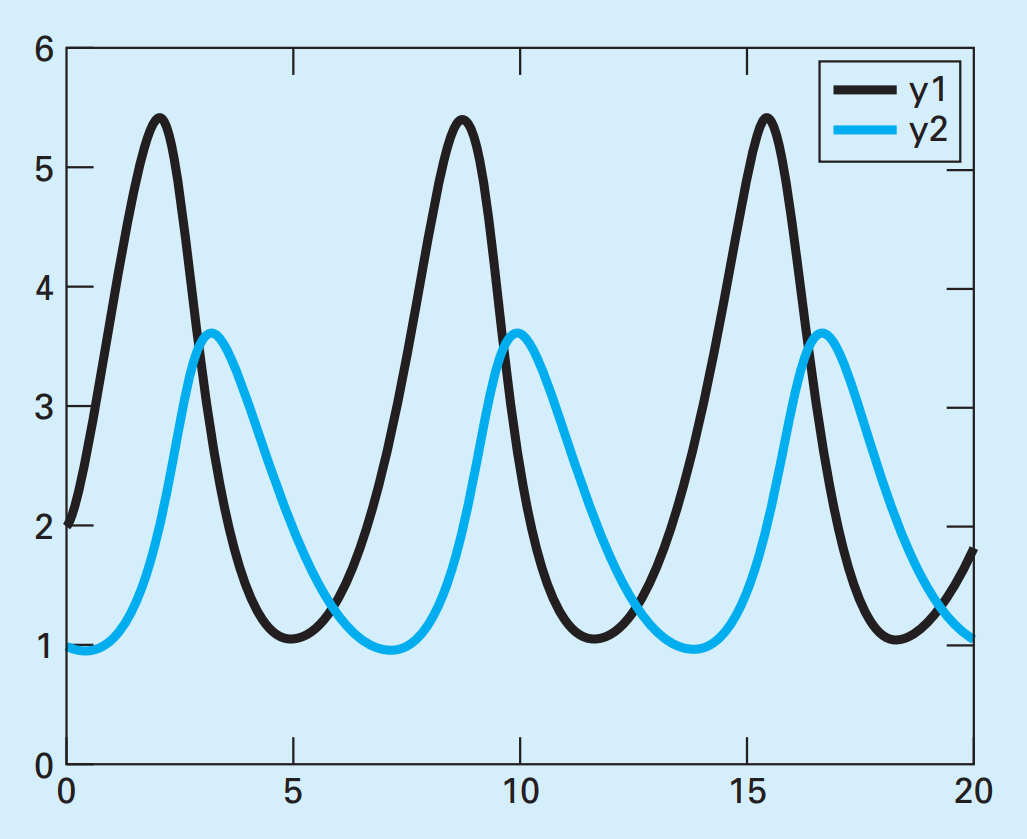
\includegraphics[scale=0.4]{fig_23_2}
   \caption{\textsf{Solution of predator-prey model with MATLAB.}}\label{fig:fig_23_2}
\end{figure}

\begin{figure}[H]
    \centering
    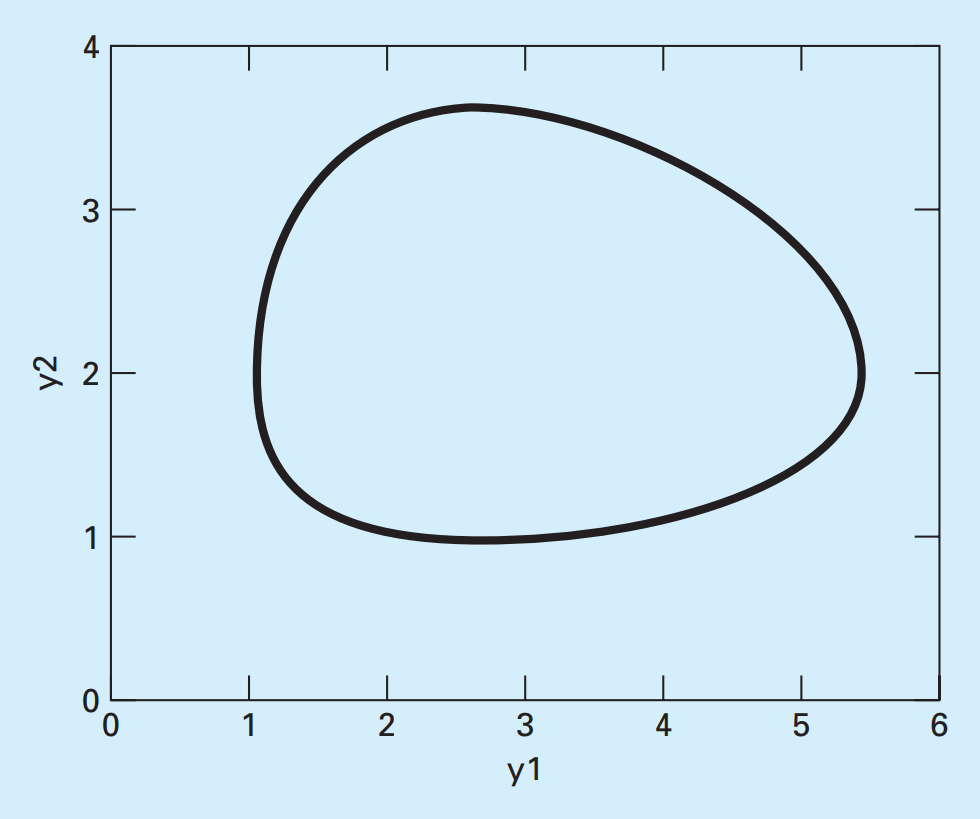
\includegraphics[scale=0.4]{fig_23_3}
   \caption{\textsf{State-space plot of predator-prey model with MATLAB.\
   }}\label{fig:fig_23_3}
\end{figure}
\end{exmp}

As in the previous example, the MATLAB solver uses default parameters to control various aspects of the integration. In addition, there is also no control over the differential equations'parameters. To have control over these features, additional arguments are included as in

\texttt{[t, y] = ode45(odefun, tspan, y0, options, p1, p2,\ldots)}\\
where  \texttt{options} is a data structure that is created with the \texttt{odeset} function to control features of the solution, and \texttt{p1, p2,\ldots} are parameters that you want to pass into odefun.

The \texttt{odeset} function has the general syntax

\texttt{options = odeset('par\textsubscript{1}',val\textsubscript{1},'par\textsubscript{2}',val\textsubscript{2},\ldots)}
where the parameter \texttt{par\textsubscript{i}} has the value \texttt{val\textsubscript{i}}. A complete listing of all the possible parameters can be obtained by merely entering \texttt{odeset} at the command prompt. Some commonly used parameters are

\texttt{'RelTol'}\indent Allows you to adjust the relative tolerance.

\texttt{'AbsTol'}\indent Allows you to adjust the absolute tolerance.

\texttt{'InitialStep'}\hspace{1mm} The solver automatically determines the initial step. This option allows you to set your own. 

\texttt{'MaxStep'}\hspace{9mm} The maximum step defaults to one-tenth of the tspan interval. This option allows you to override this default.

\begin{example}\textbf{Using \texttt{odeset} to Control Integartions Options.}

    \noindent\textit{Problem Statement} \quad Use \texttt{ode23} to solve the following ODE from $t$ = 0 to 4:
        \begin{equation}
        \frac{d y}{d t}=10 e^{-(t-2)^{2} /\left[2(0.075)^{2}\right]}-0.6 y  \nonumber
    \end{equation} 
\noindent where y(0) = 0.5. Obtain solutions for the default (10\textsuperscript{-3}) and for a more stringent (10\textsuperscript{-4}) relative error tolerance.

\noindent\textit{Solution.} First, we will create an M-file to compute the right-hand side of the ODE:\

\texttt{function yp = dydt(t, y)}

\texttt{yp = 10*exp(-(t-2)*(t-2)/(2*.075\^{}2))-0.6*y}

\noindent Then, we can implement the solver without setting the options. Hence the default value for
the relative error (10\textsubscript{-3}) is automatically used:

\texttt{>> ode23(@dydt, [0 4], 0.5);}

\noindent Note that we have not set the function equal to output variables \texttt{[t, y]}. When we implement one of the ODE solvers in this way, MATLAB automatically creates a plot of the
results displaying circles at the values it has computed. As in Fig. 23.4a, notice how \texttt{ode23}
takes relatively large steps in the smooth regions of the solution whereas it takes smaller
steps in the region of rapid change around $t$ = 2.
We can obtain a more accurate solution by using the odeset function to set the relative error tolerance to 10\textsuperscript{-4}:

\texttt{>> options=odeset('RelTol',1e-4);}

\texttt{>> ode23(@dydt, [0, 4], 0.5, options);}

\noindent As in Fig. 23.4$b$, the solver takes more small steps to attain the increased accuracy.

\begin{figure}[H]
    \centering
    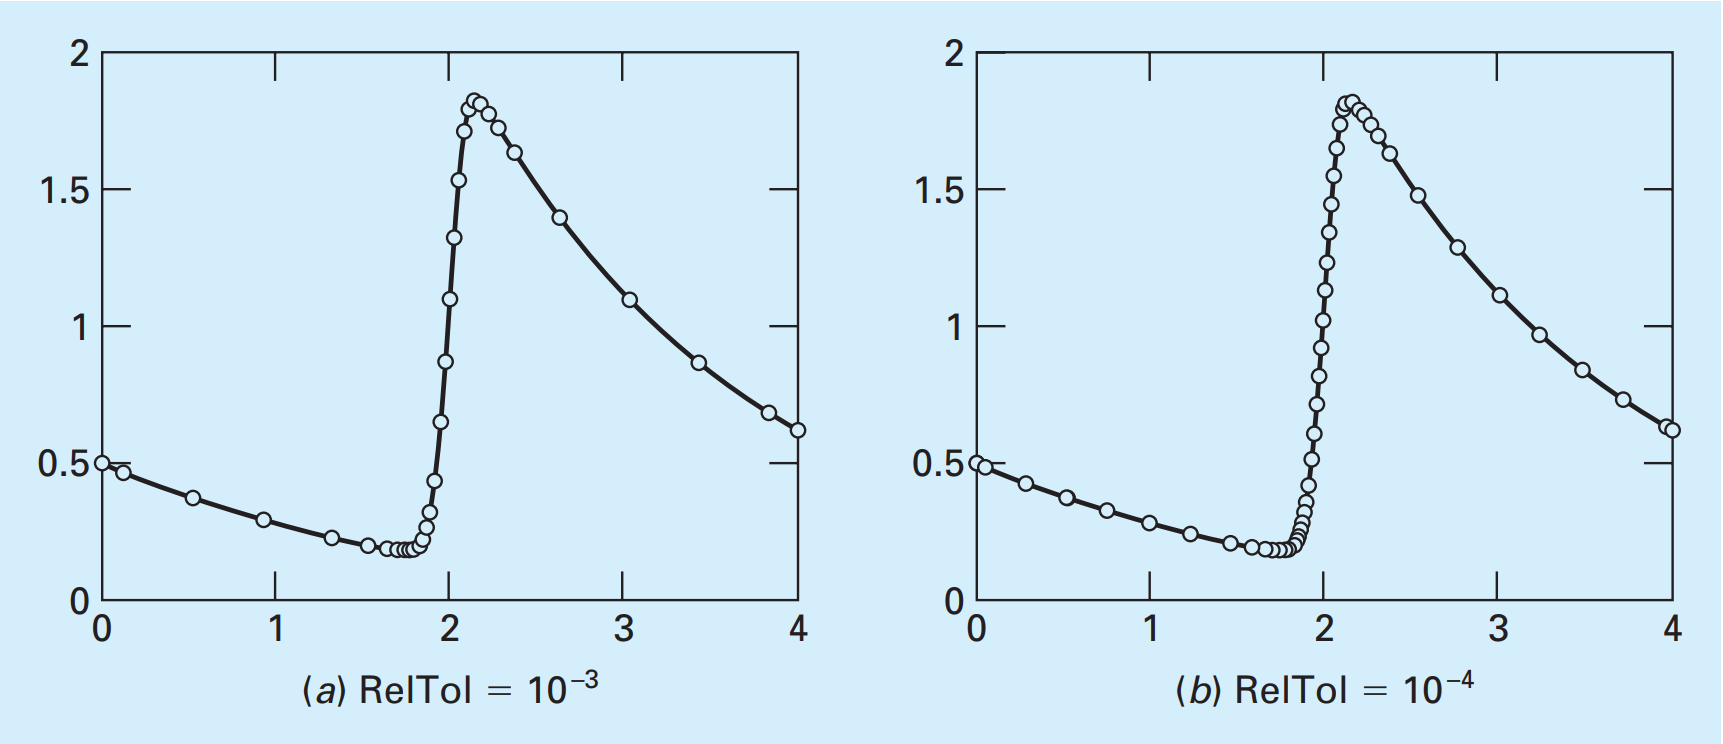
\includegraphics[scale=0.4]{fig_23_4}
   \caption{\textsf{Solution of ODE with MATLAB. For (b), a smaller relative error tolerance is used and hence many
   more steps are taken.}}\label{fig:fig_23_4}
\end{figure}
\end{example}

\subsection{Events}
MATLAB's ODE solvers are commonly implemented for a prespecified integration interval. That is, they are often used to obtain a solution from an initial to a final value of the dependent variable. However, there are many problems where we do not know the final time.

A nice example relates to the free-falling bungee jumper that we have been using
throughout this book. Suppose that the jump master inadvertently neglects to attach the cord to the jumper. The final time for this case, which corresponds to the jumper hitting the ground, is not a given. In fact, the objective of solving the ODEs would be to determine when the jumper hit the ground.

MATLAB's \texttt{events} option provides a means to solve such problems. It works by
solving differential equations until one of the dependent variables reaches zero. Of course, there may be cases where we would like to terminate the computation at a value other than zero. As described in the following paragraphs, such cases can be readily accommodated.

We will use our bungee jumper problem to illustrate the approach. The system of
ODEs can be formulated as

\begin{equation}
    \begin{aligned}
    \frac{d x}{d t} &=v \\
    \frac{d v}{d t} &=g-\frac{c_{d}}{m} v|v| \nonumber
    \end{aligned}
\end{equation}


\noindent where $x$ = distance (m), $t$ = time (s), $v$ = velocity (m/s) where positive velocity is in the downward direction, $g$ = the acceleration of gravity (= 9.81 m/s\textsuperscript{2}), c\textsubscript{d} = a second-orderdrag coefficient (kg/m), and $m$ = mass (kg).
Note that in this formulation, distance andvelocity are both positive in the downward direction, and the ground level is defined aszero distance. For the present example, we will assume that the jumper is initially located 200 m above the ground and the initial velocity is 20 m/s in the upward direction-that is, x(0) = -200 and v(0) = -20.

The first step is to express the system ODEs as an M-File function:

\texttt{function dydt=freeall (t, y, cd, m)}

\texttt{\% y(1) = x and y(2) = v}

\texttt{grav=9.81;}

\texttt{dydt=[y(2);grav-cd/m*y(2)*abs(y(2))];}

\noindent In order to implement the event, two other M-files need to be developed. These are (1) a function that defines the event, and (2) a script that generates the solution.

For our bungee jumper problem, the event function (which we have named \texttt{endevent}) can be written as

\texttt{function [detect,stopint,direction]=endevent(t,y,varargin)}

\texttt{\% Locate the time when height passes through zero}

\texttt{\% and stop integration.}

\texttt{detect=y(1); \quad \% Detect height = 0}

\texttt{stopint=1; \quad \% Stop the integration}

\texttt{direction=0; \quad \% Direction does not matter}

\noindent This function is passed the values of the independent (\texttt{t}) and dependent variables (\texttt{y}) along
with the model parameters (\texttt{varargin}). It then computes and returns three variables.
The first, \texttt{detect}, specifies that MATLAB should detect the event when the dependent
variable \texttt{y(1)} equals zero-that is, when the height x = 0. The second, \texttt{stopint}, is set to 1.
This instructs MATLAB to stop when the event occurs. The final variable, \texttt{direction}, is set to 0 if all zeros are to be detected (this is the default), +1 if only the zeros where the
event function increases are to be detected, and -1 if only the zeros where the event function decreases are to be detected. In our case, because the direction of the approach to zero
is unimportant, we set \texttt{direction} to zero.\footnote[1]{Note that, as mentioned previously, we might want to detect a nonzero event. For example, we might want to
detect when the jumper reached x = 5. To do this, we would merely set detect = y(1) - 5.}

Finally, a script can be developed to generate the solution:

\texttt{opts=odeset('events',@endevent);\\
\indent y0=[-200 -20];\\
\indent [t,y,te,ye]=ode45(@freefall,[0 inf],y0,opts,0.25,68.1);\\
\indent te,ye\\
\indent plot(t,-y(:,1),'-',t,y(:,2),'--','LineWidth',2)\\
\indent legend('Height (m)','Velocity (m/s)')\\
\indent xlabel('time (s)');\\
\indent ylabel('x (m) and v (m/s)')}

\noindent In the first line, the \texttt{odeset} function is used to invoke the \texttt{events} option and specify that the event we are seeking is defined in the \texttt{endevent} function. Next, we set the initial conditions (\texttt{y0}) and the integration interval (\texttt{tspan}).
Observe that because we do not know when the
jumper will hit the ground, we set the upper limit of the integration interval to infinity.
The third line then employs the \texttt{ode45} function to generate the actual solution. As in all of
MATLAB's ODE solvers, the function returns the answers in the vectors \texttt{t} and \texttt{y}. In addition,
when the \texttt{events} option is invoked, \texttt{ode45} can also return the time at which the event occurs
(\texttt{te}), and the corresponding values of the dependent variables (\texttt{ye}). The remaining lines of the script merely display and plot the results. When the script is run, the output is displayed as

\texttt{te =\\
\indent\indent 9.5475\\
\indent ye =\\
\indent\indent 0.0000 \indent 46.2425}

\noindent The plot is shown in Fig. 23.5. Thus, the jumper hits the ground in 9.5475 s with a velocity of 46.2454 m/s.

\begin{figure}[H]
    \centering
    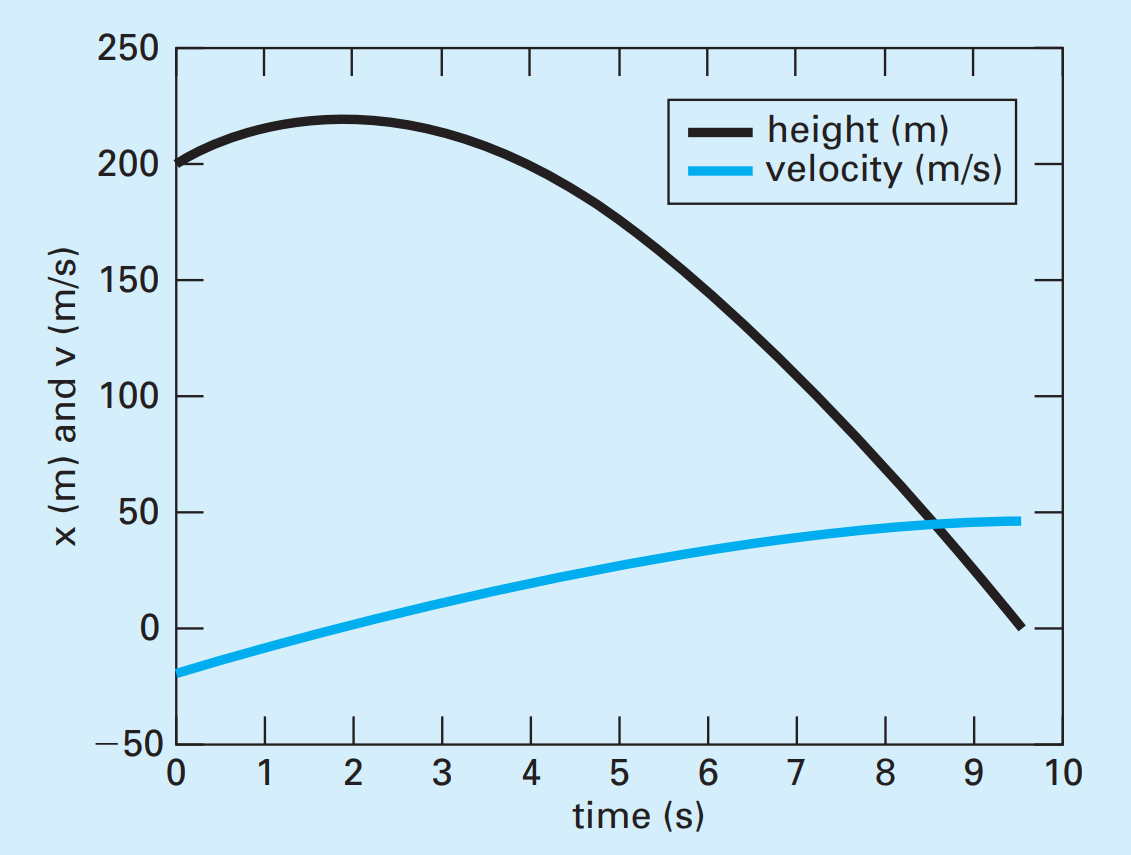
\includegraphics[scale=0.4]{fig_23_5}
   \caption{\textsf{MATLAB-generated plot of the height above the ground and velocity of the free-falling bungee jumper without the cord.}}\label{fig:fig_23_5}
\end{figure}



\vspace{2cm}
\section{Multistep methods}

The one-step methods described in the previous sections utilize information at a single
point $t$\textsubscript{i} to predict a value of the dependent variable $y$\textsubscript{i+1} at a future point $t$\textsubscript{i+1} (Fig. 23.6a).
Alternative approaches, called \textit{multistep methods} (Fig. 23.6b), are based on the insight that,
once the computation has begun, valuable information from previous points is at our
command. The curvature of the lines connecting these previous values provides information regarding the trajectory of the solution. Multistep methods exploit this information to
solve ODEs. In this section, we will present a simple second-order method that serves to
demonstrate the general characteristics of multistep approaches.

\begin{figure}[H]
    \centering
    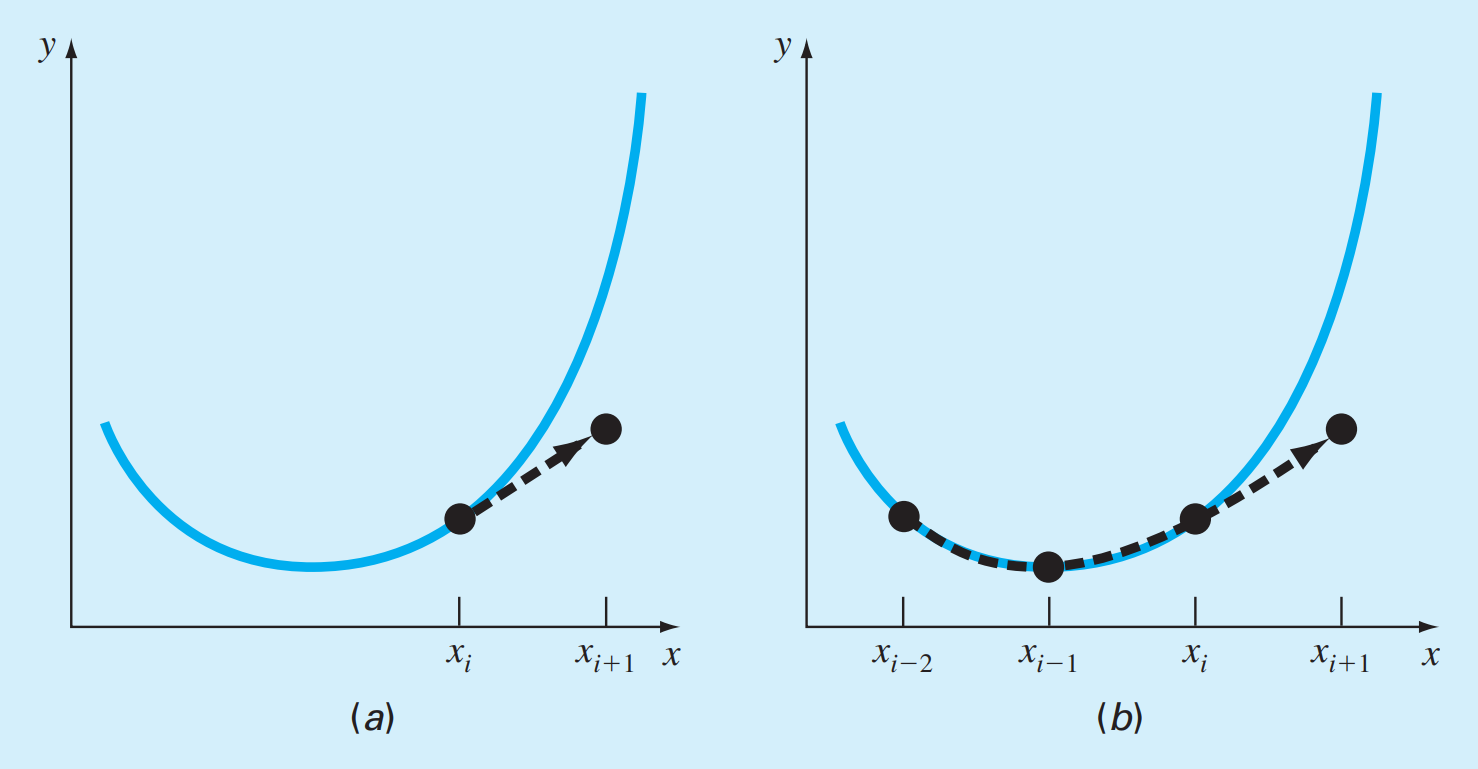
\includegraphics[scale=0.35]{fig_23_6}
   \caption{\textsf{Graphical depiction of the fundamental difference between (a) one-step and (b) multistep 
   methods for solving ODEs.}}\label{fig:fig_23_6}
\end{figure}

\subsection{The Non-Self-Starting Heun Method}
Recall that the Heun approach uses Euler's method as a predictor [Eq. (22.15)]:
\begin{equation}
    \tag{23.4}
    y_{i+1}^{0}=y_{i}+f\left(t_{i}, y_{i}\right) h
\end{equation}
and the trapezoidal rule as a corrector [Eq. (22.17)]:
\begin{equation}\tag
    {23.5}
    y_{i+1}=y_{i}+\frac{f\left(t_{i}, y_{i}\right)+f\left(t_{i+1}, y_{i+1}^{0}\right)}{2} h
\end{equation}

Thus, the predictor and the corrector have local truncation errors of O(h\textsuperscript{2}) and O(h\textsuperscript{3}),
respectively. This suggests that the predictor is the weak link in the method because it has
the greatest error. This weakness is significant because the efficiency of the iterative corrector step depends on the accuracy of the initial prediction. Consequently, one way to improve Heun's method is to develop a predictor that has a local error of O(h\textsuperscript{3}). This can be accomplished by using Euler's method and the slope at \textit{y\textsubscript{i}}, and extra information from a previous point \textit{y\textsubscript{i-1}}, as in
\begin{equation}
    \tag{23.6}
    y_{i+1}^{0}=y_{i-1}+f\left(t_{i}, y_{i}\right) 2 h
\end{equation}

\noindent This formula attains O(h\textsuperscript{3}) at the expense of employing a larger step size $2h$. In addition,
note that the equation is not self-starting because it involves a previous value of the dependent variable y\textsubscript{i-1}. Such a value would not be available in a typical initial-value problem.
Because of this fact, Eqs. (23.5) and (23.6) are called the \textit{non-self-starting Heun method}.
As depicted in Fig. 23.7, the derivative estimate in Eq. (23.6) is now located at the midpoint
rather than at the beginning of the interval over which the prediction is made. This centering improves the local error of the predictor to O(h\textsuperscript{3}).

\begin{figure}[H]
    \centering
    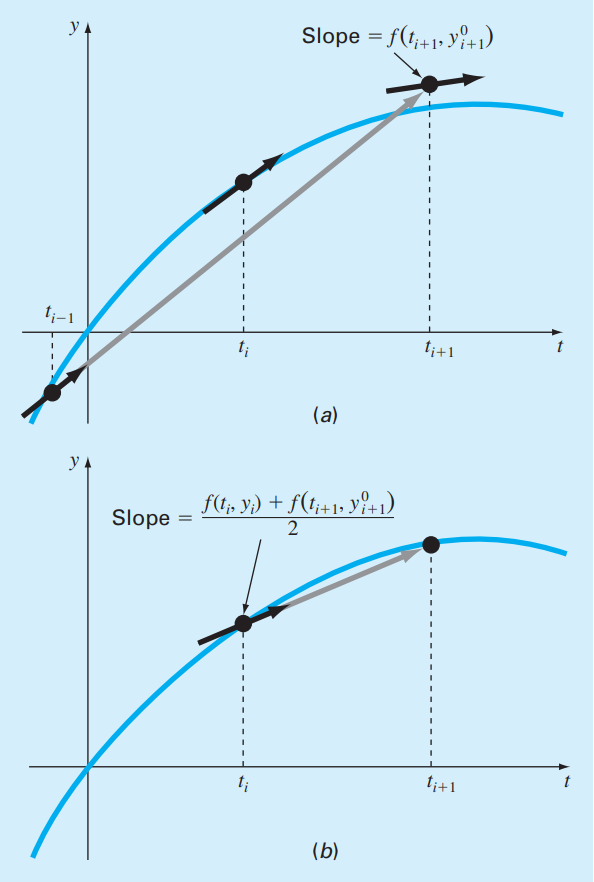
\includegraphics[scale=0.5]{fig_23_7}
   \caption{\textsf{A graphical depiction of the non-self-starting Heun method. (a) The midpoint method that is used as a predictor. (b) The trapezoidal rule that is employed as a corrector.}}\label{fig:fig_23_7}
\end{figure}
\noindent The non-self-starting Heun method can be summarized as

\noindent Predictor (Fig. 23.7a):
\begin{equation}
    \tag{23.7}
    y_{i+1}^{0}=y_{i-1}^{m}+f\left(t_{i}, y_{i}^{m}\right) 2 h
\end{equation}


\noindent Corrector (Fig. 23.7b):
\begin{equation}
    \tag{23.8}
    y_{i+1}^{j}=y_{i}^{m}+\frac{f\left(t_{i}, y_{i}^{m}\right)+f\left(t_{i+1}, y_{i+1}^{j-1}\right)}{2} h
\end{equation}
\begin{flushright}
    (for j = 1, 2,\ldots, m)
\end{flushright}

\noindent where the superscripts denote that the corrector is applied iteratively from $j = 1$ to $m$ to
obtain refined solutions. Note that $y_i^m$ and $y_{i-1}^m$ are the final results of the corrector
iterations at the previous time steps. The iterations are terminated based on an estimate of the approximate error,

\begin{equation}\
    \tag{23.9}
    \left|\varepsilon_{a}\right|=\left|\frac{y_{i+1}^{j}-y_{i+1}^{j-1}}{y_{i+1}^{j}}\right| \times 100 \%
\end{equation}

\noindent When $|\varepsilon_a|$ is less than a prespecified error tolerance $\varepsilon_s$, the iterations are terminated. At this point, $j = m$. The use of Eqs. (23.7) through (23.9) to solve an ODE is demonstrated in the following example.

\begin{exmp}
    \textbf{Non-Self-Starting Heun's Method}

    \noindent \textit{Problem statement.} Use the non-self-starting Heun method to perform the same computations as were performed previously in Example 22.2 using Heun's method. That is,
    integrate $y' = 4e\textsuperscript{0.8t} - 0.5y$ from $t = 0$ to 4 with a step size of 1. As with Example 22.2,
    the initial condition at $t$ = 0 is $y$ = 2. However, because we are now dealing with a multistep method, we require the additional information that y is equal to - 0.3929953 at $t$ = -1

    \noindent \textbf{Solution: }  The predictor [Eq. (23.7)] is used to extrapolate linearly from t = -1 to 1:
    \begin{equation}
        y_{1}^{0}=-0.3929953+\left[4 e^{0.8(0)}-0.5(2)\right] 2=5.607005 \nonumber
    \end{equation}

    \noindent The corrector [Eq. (23.8)] is then used to compute the value:
    \begin{equation}
        y_{1}^{1}=2+\frac{4 e^{0.8(0)}-0.5(2)+4 e^{0.8(1)}-0.5(5.607005)}{2} 1=6.549331 \nonumber
    \end{equation}

    \noindent which represents a true percent relative error of -5.73\% (true value = 6.194631). This
    error is somewhat smaller than the value of -8.18\% incurred in the self-starting Heun.

    Now, Eq. (23.8) can be applied iteratively to improve the solution:

    \begin{equation}
        y_{1}^{2}=2+\frac{3+4 e^{0.8(1)}-0.5(6.549331)}{2} 1=6.313749 \nonumber
    \end{equation}

    \noindent which represents an error of -1.92\%. An approximate estimate of the error can be determined using Eq. (23.9):

    \begin{equation}
        \left|\varepsilon_{a}\right|=\left|\frac{6.313749-6.549331}{6.313749}\right| \times 100 \%=3.7 \% \nonumber
    \end{equation}

    \noindent Equation (23.8) can be applied iteratively until $\varepsilon_{a}$ falls below a prespecified value of $\varepsilon_{s}$. As as the case with the Heun method (recall Example 22.2), the iterations converge on a
    value of 6.36087 ($\varepsilon_{t} = -2.68\%$). However, because the initial predictor value is more
    accurate, the multistep method converges at a somewhat faster rate.

    For the second step, the predictor is

    \begin{equation}
        y_{2}^{0}=2+\left[4 e^{0.8(1)}-0.5(6.36087)\right] 2=13.44346 \quad \varepsilon_{t}=9.43 \% \nonumber
    \end{equation}

    \noindent which is superior to the prediction of 12.0826 ($\varepsilon_{t} = 18\%$) that was computed with the original Heun method. The first corrector yields 15.76693 ($\varepsilon_{t} = 6.8\%$), and subsequent
    iterations converge on the same result as was obtained with the self-starting Heun method:
    15.30224 ($\varepsilon_{t} = -3.09\%$). As with the previous step, the rate of convergence of the corrector is somewhat improved because of the better initial prediction.
\end{exmp}


\subsection{Error estimates}

Aside from providing increased efficiency, the non-self-starting Heun can also be used to
estimate the local truncation error. As with the adaptive RK methods in Section 23.1, the
error estimate then provides a criterion for changing the step size.

The error estimate can be derived by recognizing that the predictor is equivalent to the
midpoint rule. Hence, its local truncation error is (Table 19.4)

\begin{equation}
    \tag{23.10}
    E_{p}=\frac{1}{3} h^{3} y^{(3)}\left(\xi_{p}\right)=\frac{1}{3} h^{3} f^{\prime \prime}\left(\xi_{p}\right)
\end{equation}

\noindent where the subscript $p$ designates that this is the error of the predictor. This error estimate can be combined with the estimate of $y_{i+1}$ from the predictor step to yield
\begin{equation}
    \tag{23.11}
    True\ value =y_{i+1}^{0}+\frac{1}{3} h^{3} y^{(3)}\left(\xi_{p}\right)
\end{equation}
By recognizing that the corrector is equivalent to the trapezoidal rule, a similar estimate of the local truncation error for the corrector is (Table 19.2)
\begin{equation}\tag{23.12}
    E_{c}=-\frac{1}{12} h^{3} y^{(3)}\left(\xi_{c}\right)=-\frac{1}{12} h^{3} f^{\prime \prime}\left(\xi_{c}\right)
\end{equation}

\noindent This error estimate can be combined with the corrector result $y_{i+1}$ to give
\begin{equation}
    \tag{23.13}
    True\ value =y_{i+1}^{m}-\frac{1}{12} h^{3} y^{(3)}\left(\xi_{c}\right)
\end{equation}

\noindent Equation (23.11) can be subtracted from Eq. (23.13) to yield
\begin{equation}
    \tag{23.14}
    0=y_{i+1}^{m}-y_{i+1}^{0}-\frac{5}{12} h^{3} y^{(3)}(\xi)
\end{equation}
where $\xi$ is now between $t_{i-1}$ and $t_{i}$. Now, dividing Eq. (23.14) by 5 and rearranging the result gives
\begin{equation}
    \tag{23.15}
    \frac{y_{i+1}^{0}-y_{i+1}^{m}}{5}=-\frac{1}{12} h^{3} y^{(3)}(\xi)
\end{equation}

\noindent Notice that the right-hand sides of Eqs. (23.12) and (23.15) are identical, with the exception of the argument of the third derivative. If the third derivative does not vary appreciably over the interval in question, we can assume that the right-hand sides are equal, and therefore, the left-hand sides should also be equivalent, as in
\begin{equation}
    \tag{23.16}
    E_{c}=-\frac{y_{i+1}^{0}-y_{i+1}^{m}}{5}
\end{equation}

\noindent Thus, we have arrived at a relationship that can be used to estimate the per-step truncation error on the basis of two quantities that are routine by-products of the computation: the predictor $\left(y_{i+1}^{0}\right)$ and the corrector $\left(y_{i+1}^{m}\right)$.

\begin{exmp}
    \textbf{Estimate of Per-Step Truncation Error}

    \noindent \textit{Problem Statement.} Use Eq. (23.16) to estimate the per-step truncation error of Example 23.3. Note that the true values at t = 1 and 2 are 6.194631 and 14.84392, respectively.

    \noindent \textbf{Solution.} At t\textsubscript{i+1} = 1, the predictor gives 5.607005 and the corrector yields 6.360865.

    \noindent These values can be substituted into Eq. (23.16) to give
    \begin{equation}
    E_{c}=-\frac{6.360865-5.607005}{5}=-0.150722 \nonumber
    \end{equation}

    \noindent which compares well with the exact error,
    \begin{equation}
    E_{t}=6.194631-6.360865=-0.1662341 \nonumber
    \end{equation}

    \noindent At $t_{i+1}=2$, the predictor gives $13.44346$ and the corrector yields $15.30224$, which can be used to compute
    \begin{equation}
    E_{c}=-\frac{15.30224-13.44346}{5}=-0.37176 \nonumber
    \end{equation}

    \noindent which also compares favorably with the exact error, $E_{t}=14.84392-15.30224=$ $-0.45831$.
\end{exmp}

The foregoing has been a brief introduction to multistep methods. Additional
information can be found elsewhere (e.g., Chapra and Canale, 2010). Although they
still have their place for solving certain types of problems, multistep methods are usually not the method of choice for most problems routinely confronted in engineering and
science. That said, they are still used. For example, the MATLAB function \texttt{ode113} is a
multistep method. We have therefore included this section to introduce you to their basic
principles.

\vspace{2cm}
\section{Stiffness}

\noindent Stiffness is a special problem that can arise in the solution of ordinary differential equations. A stiff system is one involving rapidly changing components together with slowly
changing ones. In some cases, the rapidly varying components are ephemeral transients
that die away quickly, after which the solution becomes dominated by the slowly varying components. Although the transient phenomena exist for only a short part of the integration
interval, they can dictate the time step for the entire solution.

\begin{figure}[H]
    \centering
    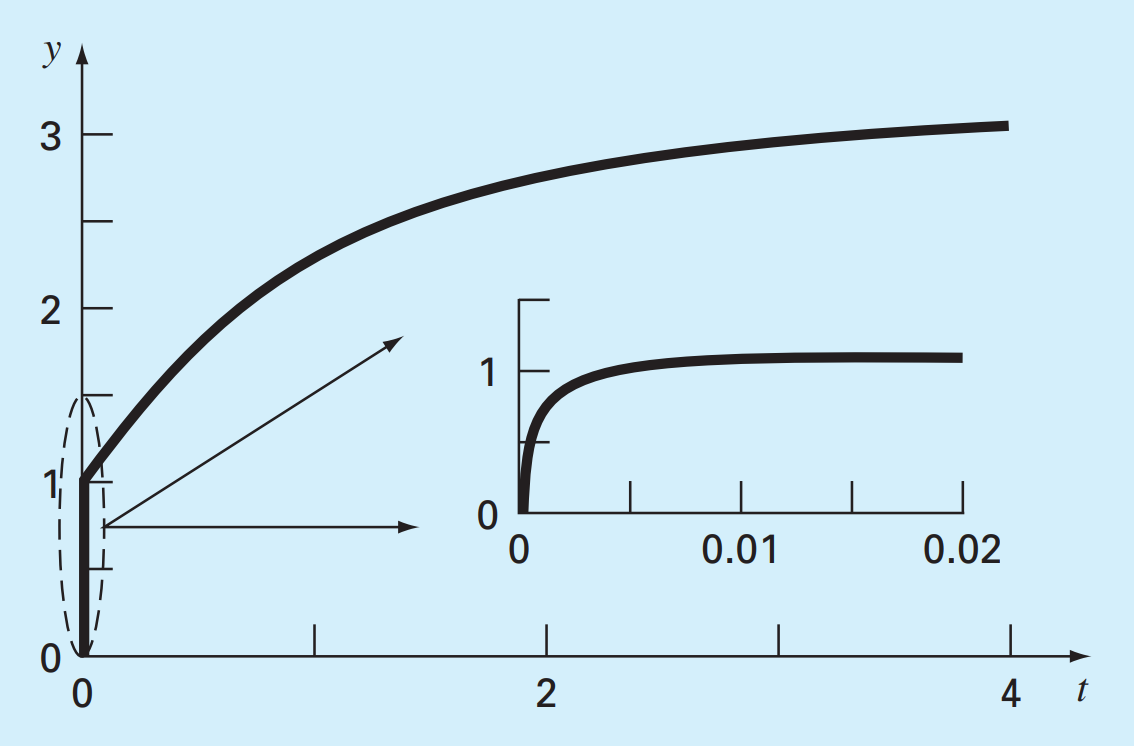
\includegraphics[scale=0.4]{fig_23_8}
   \caption{\textsf{Plot of a stiff solution of a single ODE. Although the solution appears to start at 1, there is
   actually a fast transient from y = 0 to 1 that occurs in less than the 0.005 time unit. This transient
   is perceptible only when the response is viewed on the finer timescale in the inset.}}\label{fig:fig_23_8}
\end{figure}

Both individual and systems of ODEs can be stiff. An example of a single stiff ODE is
\begin{equation}
    \tag{23.17}
    \frac{d y}{d t}=-1000 y+3000-2000 e^{-t}
\end{equation}

\noindent If $y(0)=0$, the analytical solution can be developed as
\begin{equation}
    \tag{23.18}
    y=3-0.998 e^{-1000 t}-2.002 e^{-t}
\end{equation}

\noindent As in Fig. 23.8, the solution is initially dominated by the fast exponential term $\left(e^{-1000 t}\right)$. After a short period $(t<0.005)$, this transient dies out and the solution becomes governed by the slow exponential $\left(e^{-t}\right)$.

Insight into the step size required for stability of such a solution can be gained by examining the homogeneous part of Eq. (23.17):
\begin{equation}
    \tag{23.19}
    \frac{d y}{d t}=-a y
\end{equation}

\noindent If $y(0)=y_{0}$, calculus can be used to determine the solution as
\begin{equation}
    y=y_{0} e^{-a t} \nonumber
\end{equation}

\noindent Thus, the solution starts at $y_{0}$ and asymptotically approaches zero.
Euler's method can be used to solve the same problem numerically:
\begin{equation}
    y_{i+1}=y_{i}+\frac{d y_{i}}{d t} h \nonumber
\end{equation}
Substituting Eq. (23.19) gives
\begin{equation}
    y_{i+1}=y_{i}-a y_{i} h \nonumber
\end{equation}

\noindent or
\begin{equation}
    \tag{23.20}
    y_{i+1}=y_i(1-ah)
\end{equation}

\noindent The stability of this formula clearly depends on the step size $h$. That is, $|1-a h|$ must be less than 1. Thus, if $h>2 / a,\left|y_{i}\right| \rightarrow \infty$ as $i \rightarrow \infty$.

For the fast transient part of Eq. (23.18), this criterion can be used to show that the step size to maintain stability must be $<2 / 1000=0.002$. In addition, we should note that, whereas this criterion maintains stability (i.e., a bounded solution), an even smaller step size would be required to obtain an accurate solution. Thus, although the transient occurs for only a small fraction of the integration interval, it controls the maximum allowable step size.

Rather than using explicit approaches, implicit methods offer an alternative remedy. Such representations are called \textit{implicit} because the unknown appears on both sides of the equation. An implicit form of Euler's method can be developed by evaluating the derivative at the future time:
\begin{equation}
    y_{i+1}=y_{i}+\frac{d y_{i+1}}{d t} h \nonumber
\end{equation}

\noindent This is called the backward, or implicit, Euler's method. Substituting Eq. (23.19) yields
\begin{equation}
    y_{i+1}=y_{i}-a y_{i+1} h \nonumber
\end{equation}

\noindent which can be solved for
\begin{equation}
    \tag{23.21}
    y_{i+1}=\frac{y_{i}}{1+a h}
\end{equation}

\noindent For this case, regardless of the size of the step, $\left|y_{i}\right| \rightarrow 0$ as $i \rightarrow \infty$. Hence, the approach is \textit{called unconditionally stable}.

\begin{exmp}
    \textbf{Explicit and Implicit Euler}

    \noindent \textit{Problem statement.} Use both the explicit and implicit Euler methods to solve Eq. (23.17), where y(0) = 0. \textbf{(a)} Use the explicit Euler with step sizes of 0.0005 and 0.0015 to solve for
    y between t = 0 and 0.006. \textbf{(b)} Use the implicit Euler with a step size of 0.05 to solve for y
    between 0 and 0.4.

    \noindent \textbf{Solution.} \quad \textbf{(a)} For this problem, the explicit Euler's method is

    \begin{equation}
        y_{i+1}=y_{i}+\left(-1000 y_{i}+3000-2000 e^{-t_{i}}\right) h \nonumber
    \end{equation}
    
    \noindent The result for $h=0.0005$ is displayed in Fig. 23.9a along with the analytical solution. Although it exhibits some truncation error, the result captures the general shape of the analytical solution. In contrast, when the step size is increased to a value just below the stability limit ( $h=0.0015$ ), the solution manifests oscillations. Using $h>0.002$ would result in a totally unstable solution-that is, it would go infinite as the solution progressed.

    \noindent \textbf{(b)} The implicit Euler's method is
    \begin{equation}
        y_{i+1}=y_{i}+\left(-1000 y_{i+1}+3000-2000 e^{-t_{i+1}}\right) h \nonumber
    \end{equation}
    
    \begin{figure}[H]
        \centering
        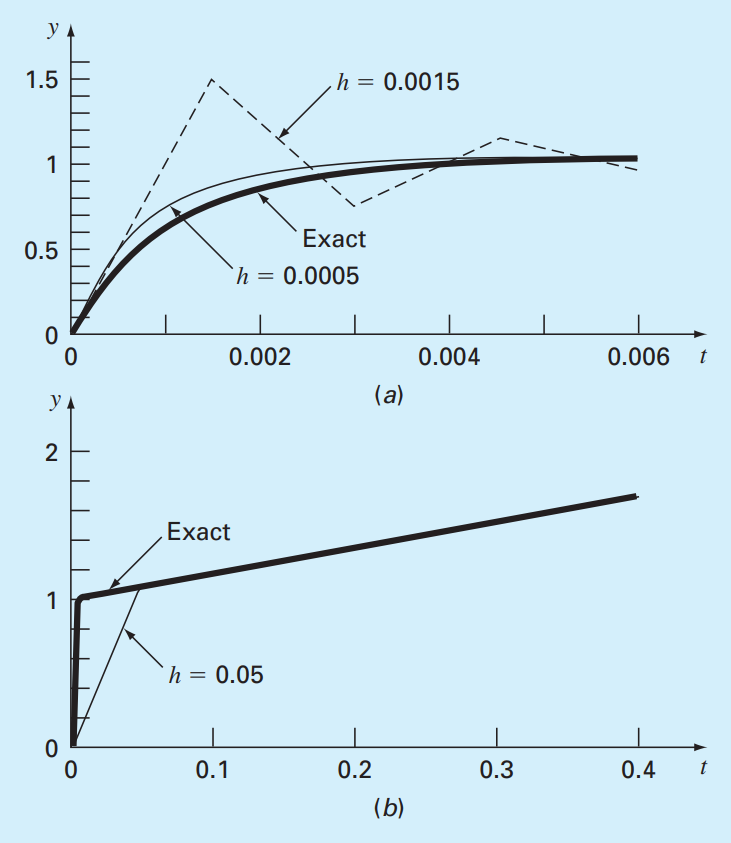
\includegraphics[scale=0.5]{fig_23_9}
       \caption{\textsf{Solution of a stiff ODE with (a) the explicit and (b) implicit Euler methods.}}\label{fig:fig_23_9}
    \end{figure}

    \noindent Now because the ODE is linear, we can rearrange this equation so that $y_{i+1}$ is isolated on the left-hand side:
    \begin{equation}
        y_{i+1}=\frac{y_{i}+3000 h-2000 h e^{-t_{i+1}}}{1+1000 h} \nonumber
    \end{equation}
    
    \noindent The result for $h=0.05$ is displayed in Fig. $23.9 b$ along with the analytical solution. Notice that even though we have used a much bigger step size than the one that induced instability for the explicit Euler, the numerical result tracks nicely on the analytical solution.
\end{exmp}
\vspace{1cm}
\noindent Systems of ODEs can also be stiff. An example is

\begin{equation}
    \tag{23.22a}
    \frac{d y_{1}}{d t}=-5 y_{1}+3 y_{2}
\end{equation}\
\begin{equation}
    \tag{23.22b}
    \frac{d y_{2}}{d t}=100 y_{1}-301 y_{2}
\end{equation}

\noindent For the initial conditions $y_{1}(0)=52.29$ and $y_{2}(0)=83.82$, the exact solution is

\begin{equation}
    \tag{23.23a}
    y_{1}=52.96 e^{-3.9899 t}-0.67 e^{-302.0101 t}
\end{equation}
\begin{equation}
    \tag{23.23b}
    y_{2}=17.83 e^{-3.9899 t}+65.99 e^{-302.0101 t}
\end{equation}

\noindent Note that the exponents are negative and differ by about two orders of magnitude. As with the single equation, it is the large exponents that respond rapidly and are at the heart of the system's stiffness.

An implicit Euler's method for systems can be formulated for the present example as

\begin{equation}
    \tag{23.24a}
    y_{1, i+1}=y_{1, i}+\left(-5 y_{1, i+1}+3 y_{2, i+1}\right) h 
\end{equation}
\begin{equation}
    \tag{23.24b}
    y_{2, i+1}=y_{2, i}+\left(100 y_{1, i+1}-301 y_{2, i+1}\right) h
\end{equation}

\noindent Collecting terms gives

\begin{equation}
    \tag{23.25a}
(1+5 h) y_{1, i+1}-3 y_{2, i+1}=y_{1, i} 
\end{equation}
\begin{equation}
    \tag{23.25b}
    -100 y_{1, i+1}+(1+301 h) y_{2, i+1}=y_{2, i}
\end{equation}

\noindent Thus, we can see that the problem consists of solving a set of simultaneous equations for each time step.

For nonlinear ODEs, the solution becomes even more difficult since it involves solving a system of nonlinear simultaneous equations (recall Sec. 12.2). Thus, although stability is gained through implicit approaches, a price is paid in the form of added solution complexity.
\texttt{}

\subsection{MATLAB Functions for Stiff Systems}

\noindent MATLAB has a number of built-in functions for solving stiff systems of ODEs. These are
\vspace{1mm}

\noindent \textbf{ode15s}. This function is a variable-order solver based on numerical differentiation formulas. It is a multistep solver that optionally uses the Gear backward differentiation formulas. This is used for stiff problems of low to medium accuracy.
\vspace{1mm}

\noindent \textbf{ode23s}. This function is based on a modified Rosenbrock formula of order 2 . Because it is a one-step solver, it may be more efficient than \texttt{ode15s} at crude tolerances. It can solve some kinds of stiff problems better than \texttt{ode15s}.
\vspace{1mm}

\noindent \textbf{ode23t}. This function is an implementation of the trapezoidal rule with a "free" interpolant. This is used for moderately stiff problems with low accuracy where you need a solution without numerical damping.
\vspace{1mm}

\noindent \textbf{ode23tb}. This is an implementation of an implicit Runge-Kutta formula with a first stage that is a trapezoidal rule and a second stage that is a backward differentiation formula of order 2 . This solver may also be more efficient than \texttt{ode15s} at crude tolerances.

\begin{exmp}
    \textbf{MATLAB for Stiff ODE's}

    \noindent \textit{Problem statement.} The van der Pol equation is a model of an electronic circuit that
    arose back in the days of vacuum tubes,

    \begin{equation}
        \tag{E23.6.1}
        \frac{d^{2} y_{1}}{d t^{2}}-\mu\left(1-y_{1}^{2}\right) \frac{d y_{1}}{d t}+y_{1}=0
    \end{equation}

    The solution to this equation becomes progressively stiffer as $\mu$ gets large. Given the initial conditions, $y_{1}(0)=d y_{1} / d t=1$, use MATLAB to solve the following two cases: \textbf{(a)} for $\mu=1$, use ode 45 to solve from $t=0$ to 20 ; and \textbf{(b)} for $\mu=1000$, use \texttt{ode23s} to solve from $t=0$ to 6000.

    \noindent \textbf{Solution.} \textbf{(a)} The first step is to convert the second-order ODE into a pair of first-order ODEs by defining

    \begin{equation}
        \frac{dy_1}{dt}=y_2 \nonumber
    \end{equation}

    \noindent Using this equation, Eq, (E23.6.1) can be written as

    \begin{equation}
        \frac{d y_{2}}{d t}=\mu\left(1-y_{1}^{2}\right) y_{2}-y_{1}=0 \nonumber 
    \end{equation}

    \noindent An M-file can now be created to hold this pair of differential equations:

    \texttt{function yp = vanderpol(t,y,mu)}

    \texttt{yp = [y(2);mu*(1-y(1)\^{}2)*y(2)-y(1)];}

    \noindent Notice how the value of $\mu$ is passed as a parameter. As in Example 23.1, \texttt{ode45} can be invoked and the results plotted:

    \noindent \texttt{>> [t,y] = ode45(@vanderpol,[0 20],[1 1],[],1);}

    \noindent \texttt{>> plot(t,y(:,1),'-',t,y(:,2),'--')}

    \noindent \texttt{>> legend('y1','y2');}

    \noindent Observe that because we are not specifying any options, we must use open brackets \texttt{[]} as
    a place holder. The smooth nature of the plot (Fig. 23.10a) suggests that the van der Pol
    equation with $\mu$ = 1 is not a stiff system.\vspace{1mm}

    \noindent \textbf{(b)} If a standard solver like ode45 is used for the stiff case ($\mu$ = 1000), it will fail miserably (try it, if you like). However, \texttt{ode23s} does an efficient job:
    \noindent \texttt{>> [t,y] = ode23s(@vanderpol,[0 6000],[1 1],[],1000);}
    \noindent \texttt{>> plot(t,y(:,1))}

    \begin{figure}[H]
        \centering
        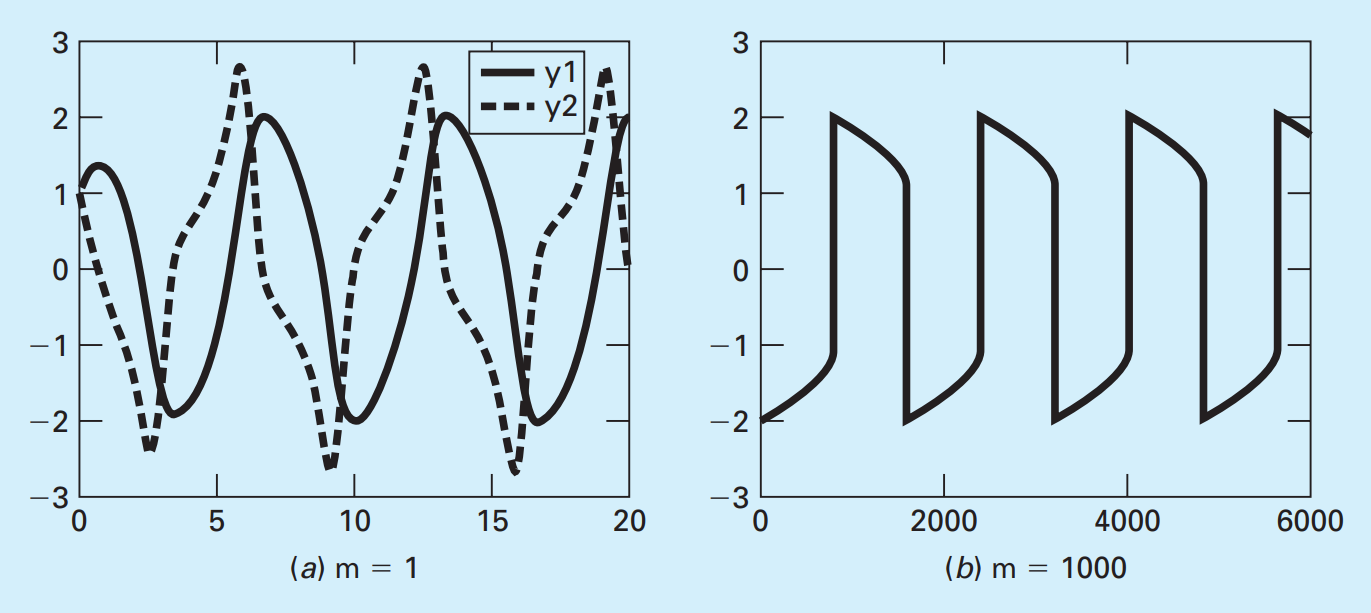
\includegraphics[scale=0.4]{fig_23_10}
       \caption{\textsf{Solutions for van der Pol's equation. (a) Nonstiff form solved with ode45 and (b) stiff form solved with \texttt{ode23s}.}}\label{fig:fig_23_10}
    \end{figure}

    We have only displayed the $y1$ component because the result for $y2$ has a much larger scale.
    Notice how this solution (Fig. 23.10b) has much sharper edges than is the case in Fig. 23.10a.
    This is a visual manifestation of the''stiffnes'' of the solution.
\end{exmp}
\vspace{10mm}


\section{MATLAB Application: Bungee Jumper with Cord}
\noindent In this section, we will use MATLAB to solve for the vertical dynamics of a jumper connected to a stationary platform with a bungee cord. As developed at the beginning of Chap. 22, the problem consisted of solving two coupled ODEs for vertical position and
velocity. The differential equation for position isolated

\begin{equation}
    \tag{23.26}
    \frac{dx}{dt} = v
\end{equation}

\noindent The differential equation for velocity is different depending on whether the jumper has fallen to a distance where the cord is fully extended and begins to stretch. Thus, if the distance
fallen is less than the cord length, the jumper is only subject to gravitational and drag forces,

\begin{equation}
    \tag{23.27a}
    \frac{d v}{d t}=g-\operatorname{sign}(v) \frac{c_{d}}{m} v^{2}
\end{equation}

\noindent Once the cord begins to stretch, the spring and dampening forces of the cord must also be included:

\begin{equation}
    \tag{23.27b}
    \frac{d v}{d t}=g-\operatorname{sign}(v) \frac{c_{d}}{m} v^{2}-\frac{k}{m}(x-L)-\frac{\gamma}{m} v
\end{equation}

\noindent The following example shows how MATLAB can be used to solve this problem.

\begin{exmp}
    \textbf{Bungee Jumper with cord}

    \noindent \textit{Problem statement.} Determine the position and velocity of a bungee jumper with the following parameters: $L=30 \mathrm{~m}, \quad g=9.81 \mathrm{~m} / \mathrm{s}^{2}, m=68.1 \mathrm{~kg}, c_{d}=0.25 \mathrm{~kg} / \mathrm{m}$, $k=40 \mathrm{~N} / \mathrm{m}$, and $\gamma=8 \mathrm{~N} \cdot \mathrm{s} / \mathrm{m}$. Perform the computation from $t=0$ to $50 \mathrm{~s}$ and assume that the initial conditions are $x(0)=v(0)=0$.

    \noindent \textbf{Solution.} The following M-file can be set up to compute the right-hand sides of the ODEs: %TODO (KOSMETYCZNE) zapisać w zwięzłej formie, w jednym "texttt{}"

    \noindent \texttt{function dydt = bungee(t,y,L,cd,m,k,gamma)}

    \noindent \texttt{g = 9.81;}
    
    \noindent \texttt{cord = 0;}

    \noindent \texttt{if y(1) > L \%determine if the cord exerts a force}

    \texttt{cord = k/m*(y(1)-L)+gamma/m*y(2);}

    \noindent \texttt{end}

    \noindent \texttt{dydt = [y(2); g - sign(y(2))*cd/m*y(2)\^{}2 - cord];}

    Because these equations are not stiff, we can use ode45 to obtain the solutions and display them on a plot:

    \noindent \texttt{>> [t,y] = ode45(@bungee,[0 50],[0 0],[],30,0.25,68.1,40,8);}

    \noindent \texttt{>> plot(t,-y(:,1),'-',t,y(:,2),':')}

    \noindent \texttt{>> legend('x (m)','v (m/s)')}

    \begin{figure}[H]
        \centering
        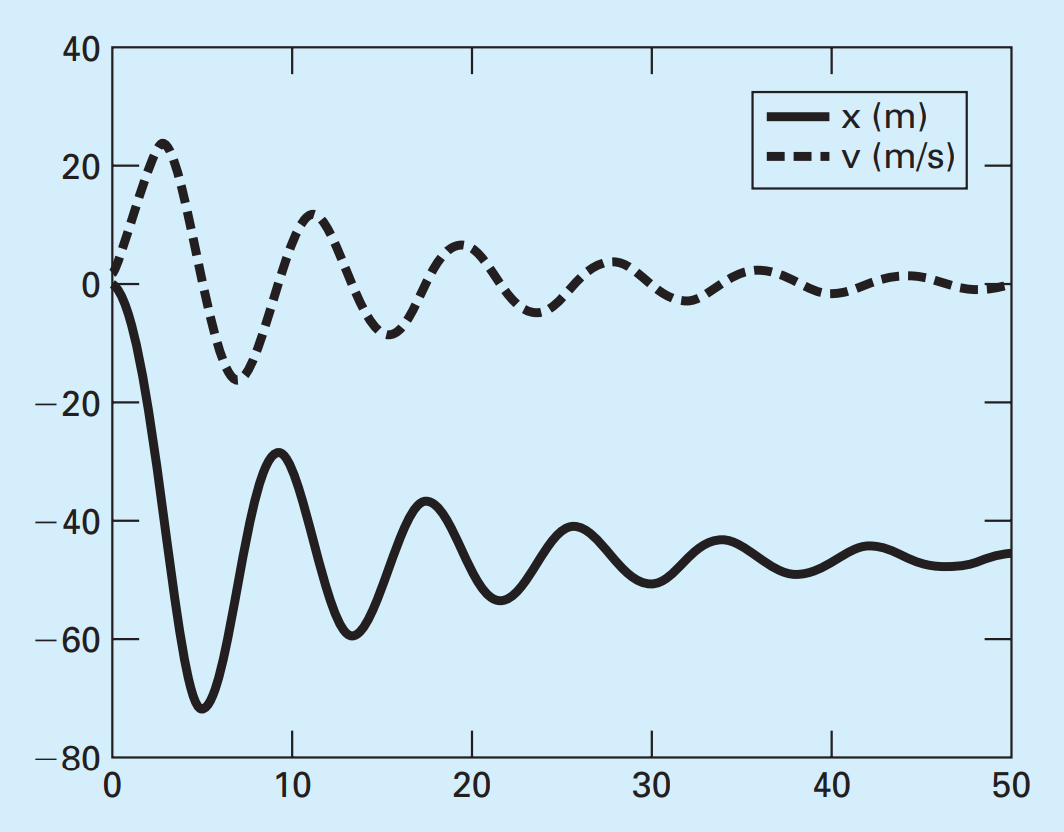
\includegraphics[scale=0.4]{fig_23_11}
       \caption{\textsf{Plot of distance and velocity of a bungee jumper.}}\label{fig:fig_23_11}
    \end{figure}
\end{exmp}
\vspace{5mm}


\section{ Case Study: Pliny's Intermittent Fountain}


\noindent \textbf{Background.} The Roman natural philosopher, Pliny the Elder, purportedly had an intermittent fountain in his garden. As in Fig. 23.12, water enters a cylindrical tank at a constant flow rate $Q_{\text {in }}$ and fills until the water reaches $y_{\text {high. }}$. At this point, water siphons out of the tank through a circular discharge pipe, producing a fountain at the pipe's exit.
The fountain runs until the water level decreases to $y_{\text {low }}$, whereupon the siphon fills with air and the fountain stops. The cycle then repeats as the tank fills until the water reaches $y_{\text {high }}$, and the fountain flows again.

When the siphon is running, the outflow $Q_{\text {out }}$ can be computed with the following formula based on Torricelli's law:
\begin{equation}
    \tag{23.28}
    Q_{\text {out }}=C \sqrt{2 g y} \pi r^{2}
\end{equation}

\begin{figure}[H]
    \centering
    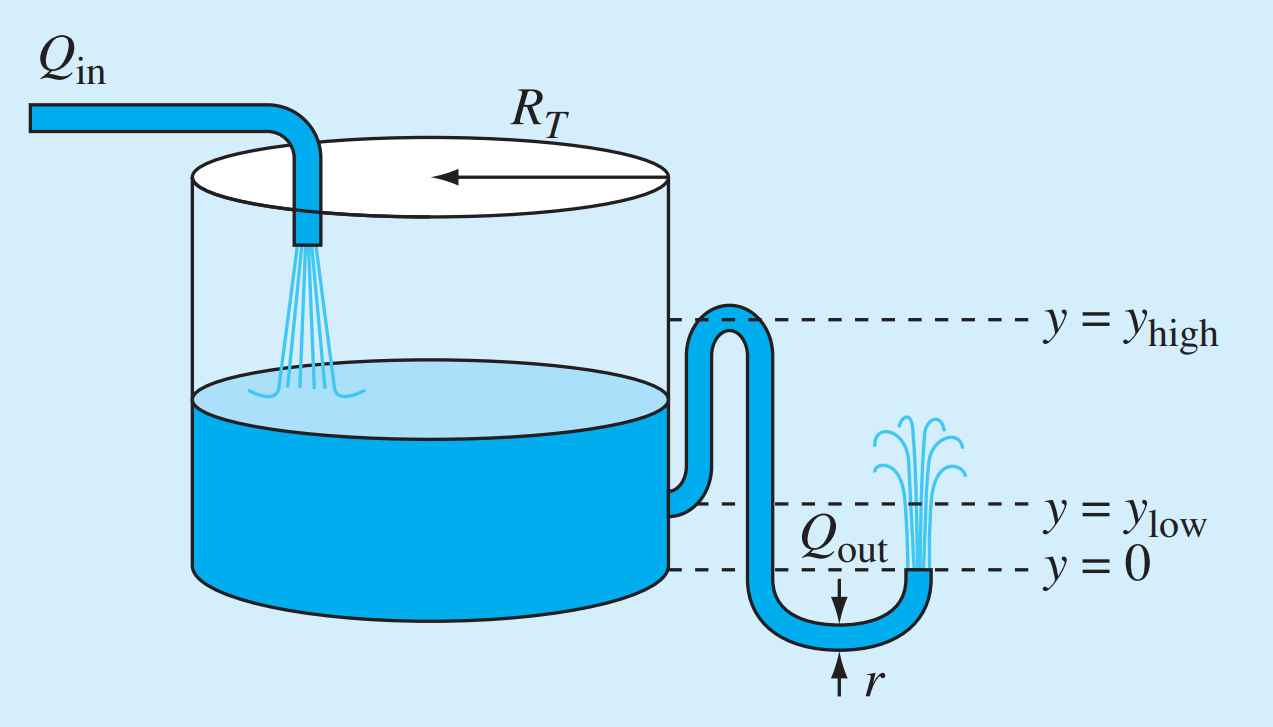
\includegraphics[scale=0.3]{fig_23_12}
   \caption{\textsf{An intermittent fountain.}}\label{fig:fig_23_12}
\end{figure}

\noindent Neglecting the volume of water in the pipe, compute and plot the level of the water in the
tank as a function of time over 100 seconds. Assume an initial condition of an empty tank
y(0) = 0, and employ the following parameters for your computation:

\begin{equation}
    \nonumber
    \begin{aligned}
    &R_{T}=0.05 \mathrm{~m} \quad r=0.007 \mathrm{~m} \quad y_{\text {low }}=0.025 \mathrm{~m}\\
    &y_{\text {high }}=0.1 \mathrm{~m} \quad C=0.6 \quad g=9.81 \mathrm{~m} / \mathrm{s}^{2}\\
    &Q_{\text {in }}=50 \times 10^{-6} \mathrm{~m}^{3} / \mathrm{s}
    \end{aligned}
\end{equation}

\noindent \textbf{Solution.} When the fountain is running, the rate of change in the tanks volume V (m\textsuperscript{3}) is determined by a simple balance of inflow minus the outflow:

\begin{equation}
    \tag{23.29}
    \frac{d V}{d t}=Q_{\text {in }}-Q_{\text {out }}
\end{equation}

\noindent where $V=$ volume $\left(\mathrm{m}^{3}\right)$. Because the tank is cylindrical, $V=\pi R_{t}^{2} y$. Substituting this relationship along with Eq. (23.28) into Eq. (23.29) gives
\begin{equation}
    \tag{23.30}
    \frac{d y}{d t}=\frac{Q_{\text {in }}-C \sqrt{2 g y} \pi r^{2}}{\pi R_{t}^{2}}
\end{equation}

When the fountain is not running, the second term in the numerator goes to zero. We can incorporate this mechanism in the model by introducing a new dimensionless variable siphon that equals zero when the fountain is off and equals one when it is flowing:
\begin{equation}
    \tag{23.31}
    \frac{d y}{d t}=\frac{Q_{\text {in }}-\operatorname{siphon} \times C \sqrt{2 g y} \pi r^{2}}{\pi R_{t}^{2}}
\end{equation}

\noindent In the present context, siphon can be thought of as a switch that turns the fountain off and on. Such two-state variables are called \textit{Boolean} or \textit{logical variables}, where zero is equivalent to false and one is equivalent to true.

Next we must relate \textit{siphon} to the dependent variable $y$. First, \textit{siphon} is set to zero whenever the level falls below $y_{\text {low. }}$. Conversely, \textit{siphon} is set to one whenever the level rises above $y_{\text {high }}$. The following M-file function follows this logic in computing the derivative:

\texttt{function dy = Plinyode(t,y)\\
\indent global siphon\\
\indent Rt = 0.05; r = 0.007; yhi = 0.1; ylo = 0.025;\\
\indent C = 0.6; g = 9.81; Qin = 0.00005;\\
\indent if y(1) <= ylo\\
\indent \vspace{\smallskipamount} siphon = 0;\\
\indent elseif y(1) >= yhi\\
\indent \vspace{\smallskipamount} siphon = 1;\\
\indent end\\
\indent Qout = siphon * C * sqrt(2 * g * y(1)) * pi * r \^{} 2;\\
\indent dy = (Qin - Qout) / (pi * Rt \^{} 2);}

\noindent Notice that because its value must be maintained between function calls, \texttt{siphon} is declared as a global variable. Although the use of global variables is not encouraged (particularly in larger programs), it is useful in the present context.

The following script employs the built-in \texttt{ode45} function to integrate \texttt{Plinyode} and
generate a plot of the solution:

\texttt{global siphon\\
\indent siphon = 0;\\
\indent tspan = [0 100]; y0 = 0;\\
\indent [tp,yp]=ode45(@Plinyode,tspan,y0);\\
\indent plot(tp,yp)\\
\indent xlabel('time, (s)')\\
\indent ylabel('water level in tank, (m)')}

As shown in Fig. 23.13, the result is clearly incorrect. Except for the original filling period, the level seems to start emptying prior to reaching $y_{\text {high }}$. Similarly, when it is draining, the siphon shuts off well before the level drops to $y_{\text {low }}$.

At this point, suspecting that the problem demands more firepower than the trusty \texttt{ode45} routine, you might be tempted to use one of the other MATLAB ODE solvers such as \texttt{ode23s} or \texttt{ode23tb}. But if you did, you would discover that although these routines yield somewhat different results, they would still generate incorrect solutions.

The difficulty arises because the ODE is discontinuous at the point that the siphon switches on or off. For example, as the tank is filling, the derivative is dependent only on the constant inflow and for the present parameters has a constant value of $6.366 \times 10^{-3} \mathrm{~m} / \mathrm{s}$.
However, as soon as the level reaches $y_{\text {high }}$, the outflow kicks in and the derivative abruptly drops to $-1.013 \times 10^{-2} \mathrm{~m} / \mathrm{s}$. Although the adaptive step-size routines used by MATLAB work marvelously for many problems, they often get heartburn when dealing with such discontinuities. Because they infer the behavior of the solution by comparing the results of different steps, a discontinuity represents something akin to stepping into a deep pothole on a dark street.

\begin{figure}[H]
    \centering
    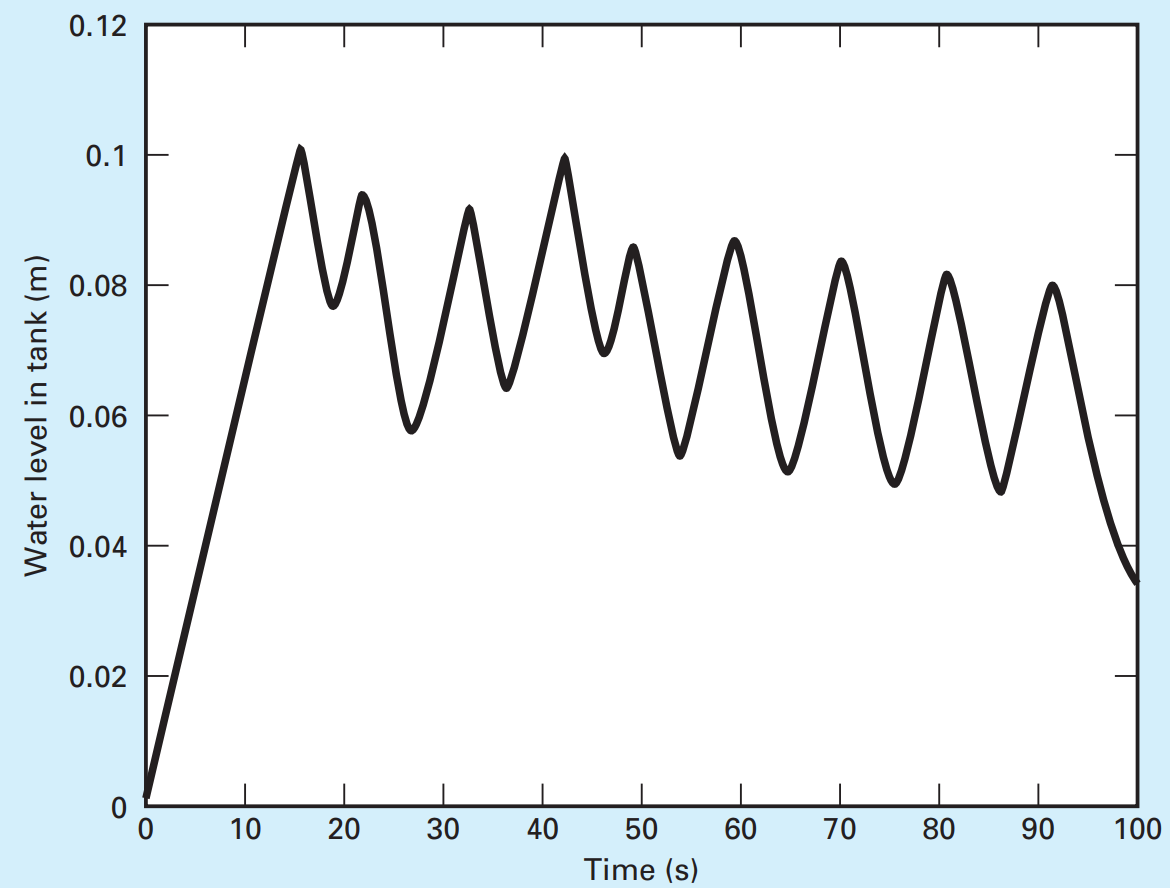
\includegraphics[scale=0.4]{fig_23_13}
   \caption{\textsf{The level in Pliny's fountain versus time as simulated with \texttt{ode45}.}}\label{fig:fig_23_13}
\end{figure}

At this point, your first inclination might be to just give up. After all, if it's too hard for
MATLAB, no reasonable person could expect you to come up with a solution. Because
professional engineers and scientists rarely get away with such excuses, your only recourse
is to develop a remedy based on your knowledge of numerical methods.

Because the problem results from adaptively stepping across a discontinuity, you
might revert to a simpler approach and use a constant, small step size. If you think about it,
that's precisely the approach you would take if you were traversing a dark, pothole-filled
street. We can implement this solution strategy by merely replacing \texttt{ode45} with the
constant-step \texttt{rk4sys} function from Chap. 22 (Fig. 22.8). For the script outlined above, the
fourth line would be formulated as

\texttt{[tp,yp] = rk4sys(@Plinyode,tspan,y0,0.0625);}

\begin{figure}[H]
    \centering
    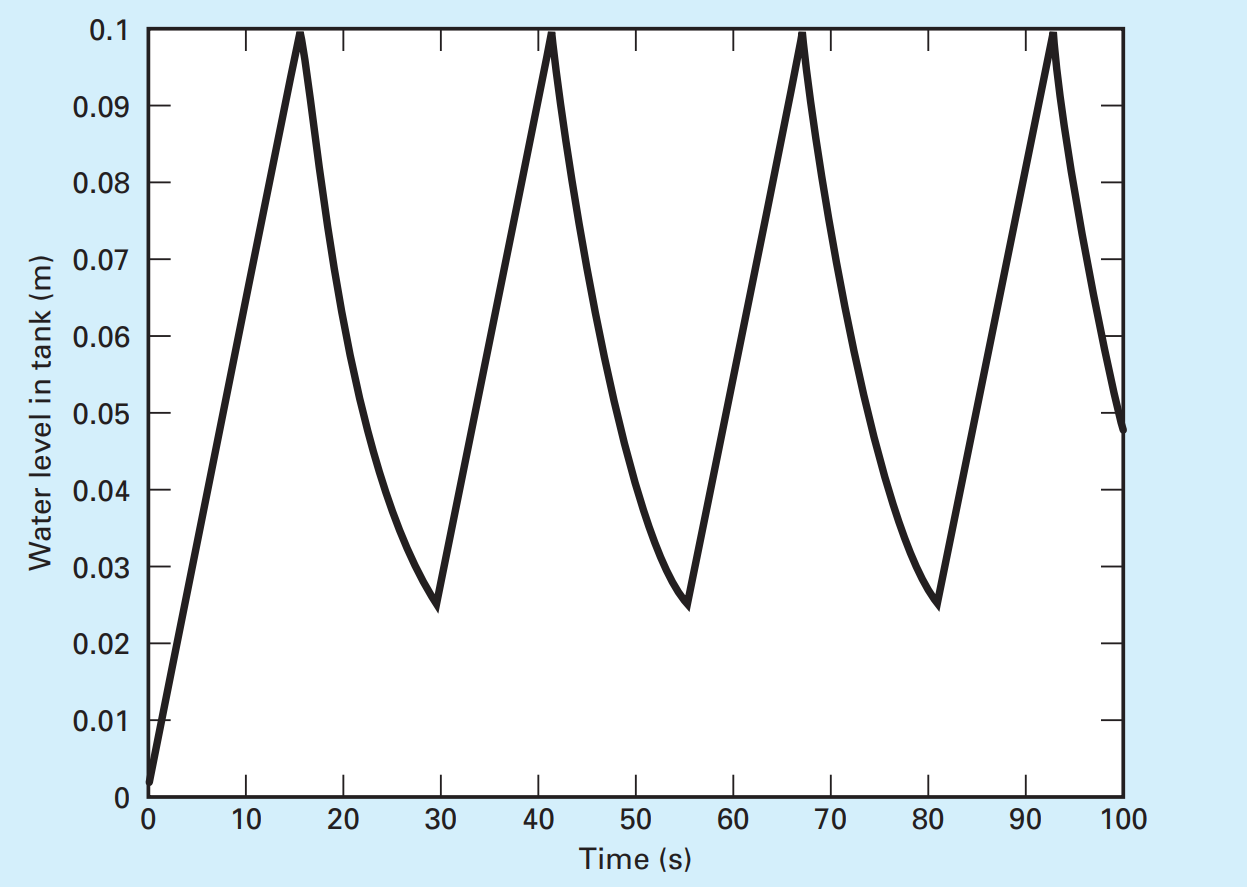
\includegraphics[scale=0.4]{fig_23_14}
   \caption{\textsf{The level in Pliny's fountain versus time as simulated with a small, constant step size using the
   \texttt{rk4sys} function (Fig. 22.8).}}\label{fig:fig_23_14}
\end{figure}

\noindent As in Fig. 23.14, the solution now evolves as expected. The tank fills to $y_{\text {high }}$ and then empties until it reaches $y_{\text {low }}$, when the cycle repeats.

There are a two take-home messages that can be gleaned from this case study. First, although it's human nature to think the opposite, simpler is sometimes better. After all, to paraphrase Einstein, "Everything should be as simple as possible, but no simpler." Second, you should never blindly believe every result generated by the computer.
You've probably heard the old chestnut, "garbage in, garbage out" in reference to the impact of data quality on the validity of computer output. Unfortunately, some individuals think that regardless of
what went in (the data) and what's going on inside (the algorithm), it's always''gospel out''
Situations like the one depicted in Fig. 23.13 are particularly dangerous-that is, although
the output is incorrect, it's not obviously wrong. That is, the simulation does not go unstable or yield negative levels. In fact, the solution moves up and down in the manner of an
intermittent fountain, albeit incorrectly.
Hopefully, this case study illustrates that even a great piece of software such as
MATLAB is not foolproof. Hence, sophisticated engineers and scientists always examine
numerical output with a healthy skepticism based on their considerable experience and
knowledge of the problems they are solving.
\vspace{5mm}
\section{PROBLEMS}

\begin{multicols}{2}
    \noindent \textbf{23.1} Repeat the same simulations as in Section $23.5$ for Pliny's fountain, but generate the solutions with \texttt{ode23}, \texttt{ode23s}, and \texttt{ode113}. Use subplot to develop a vertical three-pane plot of the time series.\vspace{2mm}

    \noindent \textbf{23.2} The following ODEs have been proposed as a model of an epidemic:
    $$
    \begin{aligned}
    \frac{d S}{d t} &=-a S I \\
    \frac{d I}{d t} &=a S I-r I \\
    \frac{d R}{d t} &=r I
    \end{aligned}
    $$
    where $S=$ the susceptible individuals, $I=$ the infected, $R=$ the recovered, $a=$ the infection rate, and     $r=$ the recovery rate. A city has 10,000 people, all of whom are susceptible.

    \noindent\textbf{(a)} If a single infectious individual enters the city at $t=0$, compute the progression of    the epidemic until the number of infected individuals falls below 10 . Use the following parameters: $a=0.002  /$ (person $\cdot$ week) and $r=0.15 / \mathrm{d}$. Develop time-series plots of all the state variables.    Also generate a phase-plane plot of $S$ versus $I$ versus $R$.

    \noindent\textbf{(b)} Suppose that after recovery, there is a loss of immunity that causes recovered    individuals to become susceptible. This reinfection mechanism can be computed as $\rho R$, where $\rho=$ the   reinfection rate. Modify the model to include this mechanism and repeat the computations in (a) using $\rho=0.    03 / \mathrm{d}$.\vspace{2mm}

    \noindent \textbf{23.3} Solve the following initial-value problem over the interval from $t=2$ to 3 :
    $$
    \frac{d y}{d t}=-0.5 y+e^{-t}
    $$
    Use the non-self-starting Heun method with a step size of $0.5$ and initial conditions of $y(1.5)=5.222138$     and $y(2.0)=4.143883$. Iterate the corrector to $\varepsilon_{s}=0.1 \%$. Compute the percent relative errors   for your results based on the exact solutions obtained analytically: $y(2.5)=3.273888$ and $y(3.0)=2.577988$. \vspace{2mm}

    \noindent \textbf{23.4} Solve the following initial-value problem over the interval from $t=0$ to $0.5$ :
    $$
    \frac{d y}{d t}=y t^{2}-y
    $$
    Use the fourth-order RK method to predict the first value at $t=0.25$. Then use the non-self-starting Heun method to make the prediction at $t=0.5$. Note: $y(0)=1$.\vspace{2mm}

    \noindent \textbf{23.5} Given
    $$
    \frac{d y}{d t}=-100,000 y+99,999 e^{-t}
    $$
    \textbf{(a)} Estimate the step size required to maintain stability using the explicit Euler method.\\
    \textbf{(b)} If $y(0)=0$, use the implicit Euler to obtain a solution from $t=0$ to 2 using a step size of $0.  1$.\vspace{2mm}

    \noindent \textbf{23.6} Given
    $$
    \frac{d y}{d t}=30(\sin t-y)+3 \cos t
    $$
    If $y(0)=0$, use the implicit Euler to obtain a solution from $t=0$ to 4 using a step size of $0.4$.\vspace {2mm}

    \noindent \textbf{23.7} Given
    $$
    \begin{aligned}
    &\frac{d x_{1}}{d t}=999 x_{1}+1999 x_{2} \\
    &\frac{d x_{2}}{d t}=-1000 x_{1}-2000 x_{2}
    \end{aligned}
    $$
    If $x_{1}(0)=x_{2}(0)=1$, obtain a solution from $t=0$ to $0.2$ using a step size of $0.05$ with the \textbf{   (a)} explicit and \textbf{(b)} implicit Euler methods.\vspace{2mm}

    \noindent \textbf{23.8} The following nonlinear, parasitic ODE was suggested by Hornbeck (1975):
    $$
    \frac{d y}{d t}=5\left(y-t^{2}\right)
    $$
    If the initial condition is $y(0)=0.08$, obtain a solution from $t=0$ to 5 :
    \textbf{(a)} Analytically.\\
    \textbf{(b)} Using the fourth-order RK method with a constant step size of $0.03125$.\\
    \textbf{(c)} Using the MATLAB function \texttt{ode45}.\\
    \textbf{(d)} Using the MATLAB function \texttt{ode23s}.\\
    \textbf{(e)} Using the MATLAB function \texttt{ode23tb}.\\
    Present your results in graphical form.\vspace{2mm}

    \noindent \textbf{23.9} Recall from Example $20.5$ that the following \texttt{humps} function exhibits both     flat and steep regions over a relatively short $x$ range,
    $$
    f(x)=\frac{1}{(x-0.3)^{2}+0.01}+\frac{1}{(x-0.9)^{2}+0.04}-6
    $$
    Determine the value of the definite integral of this function between $x=0$ and 1 using \textbf{(a)} the \texttt{quad} and \textbf{(b)} the \texttt{ode45} functions.\vspace{2mm}

    \noindent\textbf{23.10} The oscillations of a swinging pendulum can be simulated with the following nonlinear   model:
    $$
    \frac{d^{2} \theta}{d t^{2}}+\frac{g}{l} \sin \theta=0
    $$
    where $\theta=$ the angle of displacement, $g=$ the gravitational constant, and $l=$ the pendulum length. For   small angular displacements, the $\sin \theta$ is approximately equal to $\theta$ and the model can be    linearized as
    $$
    \frac{d^{2} \theta}{d t^{2}}+\frac{g}{l} \theta=0
    $$
    Use \texttt{ode45} to solve for $\theta$ as a function of time for both the linear and nonlinear models where   $l=0.6 \mathrm{~m}$ and $g=9.81 \mathrm{~m} / \mathrm{s}^{2}$. First, solve for the case where the initial    condition is for a small displacement $(\theta=\pi / 8$ and $d \theta / d t=0)$. Then repeat the calculation   for a large displacement $(\theta=\pi / 2)$. For each case, plot the linear and nonlinear simulations on the  same plot.\vspace{2mm}

    \noindent\textbf{23.11} Employ the events option described in Section $23.1 .2$ to determine the period of a    $1-\mathrm{m}$ long, linear pendulum (see description in Prob. 23.10). Compute the period for the following    initial conditions: \textbf{(a)} $\theta=\pi / 8$, \textbf{(b)} $\theta=\pi / 4$, and \textbf{(c)}     $\theta=\pi / 2$.
    For all three cases, set the initial angular velocity at zero. (\textbf{Hint:} A good way to compute the    period is to determine how long it takes for the pendulum to reach $\theta=0$ [i.e., the bottom of its arc]).  The period is equal to four times this value.\vspace{2mm}

    \noindent\textbf{23.12} Repeat Prob. 23.11, but for the nonlinear pendulum described in Prob. 23.10.\vspace {2mm}

    \noindent\textbf{23.13} The following system is a classic example of stiff ODEs that can occur in the   solution of chemical reaction kinetics:
    $$
    \begin{aligned}
    \frac{d c_{1}}{d t} &=-0.013 c_{1}-1000 c_{1} c_{3} \\
    \frac{d c_{2}}{d t} &=-2500 c_{2} c_{3} \\
    \frac{d c_{3}}{d t} &=-0.013 c_{1}-1000 c_{1} c_{3}-2500 c_{2} c_{3}
    \end{aligned}
    $$
    Solve these equations from $t=0$ to 50 with initial conditions $c_{1}(0)=c_{2}(0)=1$ and $c_{3}(0)=0$. If you   have access to MATLAB software, use both standard (e.g., \texttt{ode45} ) and stiff (e.g., \texttt{ode23s} )  functions to obtain your solutions.\vspace{2mm}

    \noindent\textbf{23.14} The following second-order ODE is considered to be stiff:
    $$
    \frac{d^{2} y}{d x^{2}}=-1001 \frac{d y}{d x}-1000 y
    $$
    Solve this differential equation (a) analytically and 
    (b) numerically for x = 0 to 5. For (b) use an implicit
    approach with h = 0.5. Note that the initial conditions are
    y(0) = 1 and $y'$(0) = 0. Display both results graphically.\vspace{2mm}

    \noindent\textbf{23.15} Consider the thin rod of length $l$ moving in the $x-y$ plane as shown in Fig. P23. 15. The rod is fixed with a pin on one end and a mass at the other. Note that $g=9.81 \mathrm{~m} / \mathrm{s}   ^{2}$ and $l=0.5 \mathrm{~m}$. This system can be solved using
    $$
    \ddot{\theta}-\frac{g}{l} \theta=0
    $$
    Let $\theta(0)=0$ and $\dot{\theta}(0)=0.25 \mathrm{rad} / \mathrm{s}$. Solve using any method studied in   this chapter. Plot the angle versus time and the angular velocity versus time. (\textbf{Hint:} Decompose the  secondorder ODE.)

    \begin{figure}[H]
        \centering
        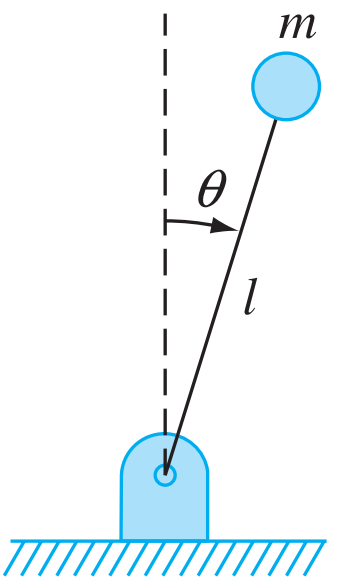
\includegraphics[scale=0.4]{fig_P_23_15}
        \caption{\textsf{}}
        \label{fig:fig_P_23_15} %TODO wyświetlanie odpowiedniego(!) podpisu obrazka
    \end{figure}\vspace{2mm}

    \noindent\textbf{23.16} Given the first-order ODE:
    $$
    \begin{aligned}
    &\frac{d x}{d t}=-700 x-1000 e^{-t} \\
    &x(t=0)=4
    \end{aligned}
    $$
    Solve this stiff differential equation using a numerical method over the time period $0 \leq t \leq 5$. Also    solve analytically and plot the analytic and numerical solution for both the fast transient and slow   transition phase of the time scale.\vspace{2mm}

    \noindent\textbf{23.17} Solve the following differential equation from $t=0$ to 2
    $$
    \frac{d y}{d t}=-10 y
    $$
    with the initial condition $y(0)=1$. Use the following techniques to obtain your solutions: \textbf{(a)}    analytically, \textbf{(b)} the explicit Euler method, and \textbf{(c)} the implicit Euler method. For \textbf{ (b)} and \textbf{(c)} use $h=0.1$ and 0.2. Plot your results.\vspace{2mm}

    \noindent\textbf{23.18} The Lotka-Volterra equations described in Section $22.6$ have been refined to include   additional factors that impact predator-prey dynamics. For example, over and above predation, prey population     can be limited by other factors such as space. Space limitation can be incorporated into the model as a     carrying capacity (recall the logistic model described in Prob. 22.5) as in
    $$
    \begin{aligned}
    \frac{d x}{d t} &=a\left(1-\frac{x}{K}\right) x-b x y \\
    \frac{d y}{d t} &=-c y+d x y
    \end{aligned}
    $$
    where $K=$ the carrying capacity. Use the same parameter values and initial conditions as in Section $22.6$     to integrate these equations from $t=0$ to 100 using \texttt{ode45}, and develop both time series and phase     plane plots of the results.
    \textbf{(a)} Employ a very large value of $K=10^{8}$ to validate that you obtain the same results as in     Section 22.6.
    \textbf{(b)} Compare \textbf{(a)} with the more realistic carrying capacity of $K=200$. Discuss your results.   \vspace{2mm}

    \noindent\textbf{23.19} Two masses are attached to a wall by linear springs (Fig. P23.19). Force balances   based on Newton's second law can be written as
    $$
    \begin{aligned}
    &\frac{d^{2} x_{1}}{d t^{2}}=-\frac{k_{1}}{m_{1}}\left(x_{1}-L_{1}\right)+\frac{k_{2}}{m_{1}}\left(x_{2}-x_{1}  -w_{1}-L_{2}\right) \\
    &\frac{d^{2} x_{2}}{d t^{2}}=-\frac{k_{2}}{m_{2}}\left(x_{2}-x_{1}-w_{1}-L_{2}\right)
    \end{aligned}
    $$
    where $k=$ the spring constants, $m=$ mass, $L=$ the length of the unstretched spring, and $w=$ the width of    the mass. Compute the positions of the masses as a function of time using the following parameter values: $k_  {1}=k_{2}=5, m_{1}=m_{2}=2$, $w_{1}=w_{2}=5$, and $L_{1}=L_{2}=2$.
    Set the initial conditions as $x_{1}=L_{1}$ and $x_{2}=L_{1}+w_{1}+L_{2}+6$. Perform the simulation from    $t=0$ to 20. Construct time-series plots of both the displacements and the velocities. In addition, produce a  phaseplane plot of $x_{1}$ versus $x_{2}$.\vspace{2mm}

    \begin{figure}[H]
        \centering
        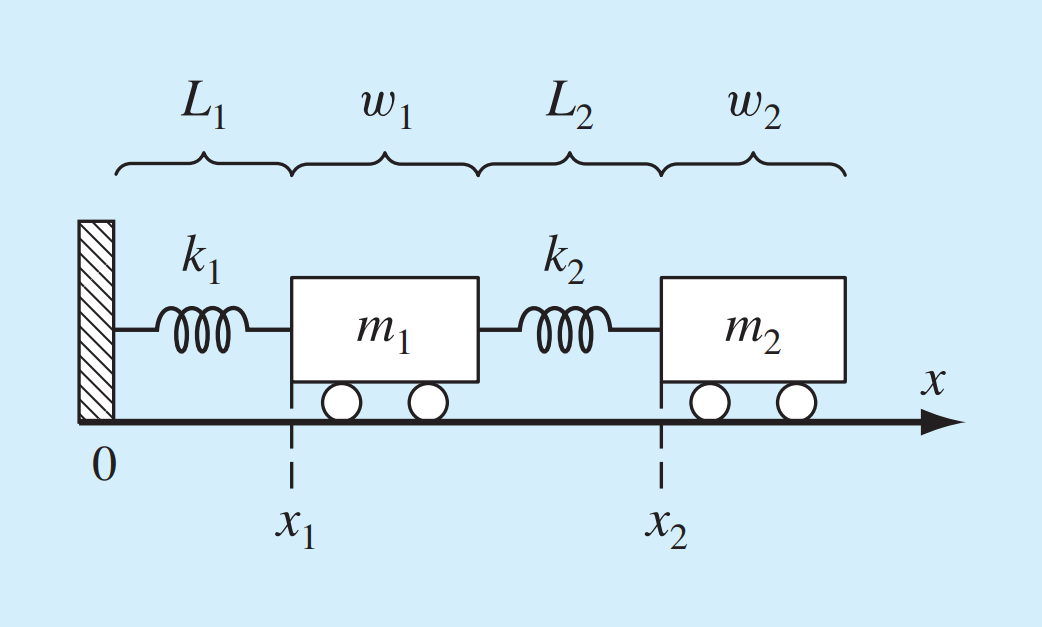
\includegraphics[scale=0.3]{fig_P_23_19}
        \caption{\textsf{}}
        \label{fig:fig_P_23_19} %TODO wyświetlanie odpowiedniego(!) podpisu obrazka
    \end{figure}\vspace{2mm}

    \noindent \textbf{23.20} Use \texttt{ode45} to integrate the differential equations for the system described    in Prob. 23.19. Generate vertically stacked subplots of displacements (top) and velocities (bottom). Employ    the \texttt{fft} function to compute the discrete Fourier transform (DFT) of the first mass's displacement.    Generate and plot a power spectrum in order to identify the system's resonant frequencies.\vspace{2mm}

    \noindent\textbf{23.21} Perform the same computations as in Prob. $23.20$ but for the structure in Prob. 22.22.

    \noindent\textbf{23.22} Use the approach and example outlined in Section 23.1.2, but determine the time, height, and velocity when the bungee jumper is the farthest above the ground, and generate a plot of the solution.

\end{multicols}

\end{document}